%(query-replace-regexp "\\\\sqsubseteq^{sh}_{\\([^}]*\\)}" "\\\\shiftpre[\\1]")
% --- LNCS ---'
\documentclass{llncs}

\usepackage{hyperref}
\usepackage[textsize=tiny]{todonotes}
\usepackage{etex}

\usepackage[all]{xy}
\SelectTips{cm}{}
% derivations and labels
\usepackage{proof}
\newcommand{\lab}[1]{\ensuremath{\mathsf{{#1}}}}
\newcommand{\slab}[1]{\ensuremath{\scriptstyle{\mathsf{{#1}}}}}

% ``boxed'' \infer command
\newcommand{\binfer}[3][]{
  \mbox{\infer[#1]{#2}{#3}}}

% Command for labels on the left side of the rule
%       \inferL{<name>}{<post>}{<pre>}
% generates:
%             <pre>
%      <name> ------
%             <post>
%
\newlength{\myheight}
\newcommand{\inferL}[3]
  {\settoheight{\myheight}{\mbox{${#2}$}}
   \raisebox{\myheight}{{#1}}
   \makebox[1mm]{}
   \mbox{\infer{#2}{#3}}
}

\usepackage{amssymb,graphicx,epsfig,color}
%\usepackage[scriptsize]{subfigure}
\usepackage{subcaption}
\usepackage{wrapfig}

% re-stating 
%\usepackage{thm-restate}

% showing labels
%\usepackage[inline]{showlabels}

\usepackage{pgf}
\usepackage{tikz}
\usepackage{tikz-cd}
\usetikzlibrary{arrows,shapes,snakes,automata,backgrounds,petri,fit,positioning}
\tikzstyle{node}=[circle, draw=black, minimum size=1mm]
\tikzstyle{trans}=[font=\scriptsize]
\tikzstyle{lab}=[font=\small]


\newcommand{\pgfBox}{
  \begin{pgfonlayer}{background} 
    \fill[blue!2,thick,draw=black!50,rounded corners,inner sep=3mm] ([xshift=-1.5pt,yshift=-1.5pt]current bounding box.south west) rectangle ([xshift=1.5pt,yshift=1.5pt]current bounding box.north east);
  \end{pgfonlayer}
}



\newcommand{\Rrel}[1]   {\stackrel{{#1}}{\Longrightarrow}}
\newcommand{\oa}{\overline a}
\newcommand{\ob}{\overline b}
\newcommand{\oc}{\overline c}
\newcommand{\od}{\overline d}
\newcommand{\nil}{{\tt 0}}
\newcommand{\rec}{\emph{rec}}
\newcommand{\fn}[1]{{\mathtt{fn}}(#1)}
%\usepackage{latexsym}
\usepackage{stmaryrd}
\def\encodep#1{\llfloor#1\rrfloor}

\newcommand{\cat}[1]{\ensuremath{\mathbf{#1}}}

\newcommand{\dpo}{\textsc{dpo}}

% base classes of categories for adhesive and quasi adhesive case
\newcommand{\bAdh}{\ensuremath{\mathbb{B}}}
\newcommand{\bQAdh}{\ensuremath{\mathbb{QB}}}

%from pawel
\usepackage[latin1]{inputenc}
\usepackage{amsmath}
%2 righe tolte da Fabio
\usepackage{amssymb}
%\usepackage{amsthm}
\usepackage{enumerate}
\usepackage{xspace}
\usepackage{amsfonts}
\usepackage{mathrsfs}
\usepackage{cite}
\usepackage{float}
\usepackage{fancybox}


%%%%%%%% MATHEMATICAL NOTATION %%%%%%%%%%%%%%%%%%%%%%%%%%%%%%%%%%%%%%%%%

%symbol for natural numbers
\newcommand{\nat}{\ensuremath{\mathbb{N}}}

% finite subset
\newcommand{\sfin}{\ensuremath{\subseteq_{\mathit{fin}}}}

% flattening of a multiset
\newcommand{\flt}[1]{\ensuremath{[\![{#1}]\!]}}

% compact elements
\newcommand{\compact}[1]{\ensuremath{\mathop{\mathsf{K}({#1})}}}

% principal ideal
\newcommand{\principal}[1]{\ensuremath{\mathop{\downarrow\!{#1}}}}

% ideal completion
\newcommand{\ideal}[1]{\ensuremath{\mathsf{Idl}({#1})}}

% complete prime elements
\newcommand{\pr}[1]{\ensuremath{\mathop{\mathit{pr}({#1})}}}
\newcommand{\wpr}[1]{\ensuremath{\mathop{\mathit{wpr}({#1})}}}

% irreducible elements
\newcommand{\ir}[1]{\ensuremath{\mathop{\mathit{ir}({#1})}}}

% difference of irreducible elements
\newcommand{\diff}[2]{\ensuremath{\delta({#1},{#2})}}

% immediate precedence

% abbreviation for event structure
% \newcommand{\esabbr}{event structure}
\newcommand{\esabbr}{\textsc{es}}
\newcommand{\esnabbr}{\textsc{esnb}}
\newcommand{\esnmabbr}{\textsc{esn}}
\newcommand{\eseqabbr}{\textsc{epes}}

% predecessor of an irreducible
\newcommand{\pred}[1]{\ensuremath{\mathit{p}({#1})}}

% irreducible elements in es domains
\newcommand{\esir}[2]{\ensuremath{\langle{#1}, {#2}\rangle}}

% equivalence classes [of irreducibles]
\newcommand{\eqclass}[2][]{\ensuremath{[{#2}]_{\scriptscriptstyle {#1}}}}
% union of the equivalence classes of the elements in a set
\newcommand{\eqclasscup}[2]{\ensuremath{{#2}_{\scriptscriptstyle {#1}}}}

\newcommand{\eqclassir}[1]{\ensuremath{\eqclass[\leftrightarrow^*]{#1}}}



% quotient of set wrt a relation
\newcommand{\quotient}[2]{\ensuremath{{#1}_{\scriptscriptstyle {#2}}}}


% category of event structures 
\newcommand{\es}{\ensuremath{\mathsf{ES}}}
% category of stable event structures 
\newcommand{\ses}{\ensuremath{\mathsf{sES}}}
% category of prime event structures 
\newcommand{\pes}{\ensuremath{\mathsf{pES}}}
% category of prime event structures with equivalence
\newcommand{\epes}{\ensuremath{\mathsf{epES}}}

% category of connected event structures 
\newcommand{\ces}{\ensuremath{\mathsf{cES}}}


% category of weak prime algebraic domains domains 
\newcommand{\WDom}{\ensuremath{\mathsf{wDom}}}
% category of domains
\newcommand{\Dom}{\ensuremath{\mathsf{Dom}}}
% category of prime algebraic domains
\newcommand{\PDom}{\ensuremath{\mathsf{pDom}}}


%%%%% NON BINARY CONFLICT

% category of event structures 
\newcommand{\esn}{\ensuremath{\mathsf{ES_{nb}}}}
% category of stable event structures 
\newcommand{\sesn}{\ensuremath{\mathsf{sES_n}}}

% category of connected event structures 
\newcommand{\cesn}{\ensuremath{\mathsf{cES_{nb}}}}

% category of prime event structures 
\newcommand{\pesn}{\ensuremath{\mathsf{pES_n}}}

% category of fusion domains 
\newcommand{\WDomb}{\ensuremath{\mathsf{wDom_b}}}
% category of domains
\newcommand{\Domb}{\ensuremath{\mathsf{Dom_b}}}
% category of prime algebraic domains
\newcommand{\PDomb}{\ensuremath{\mathsf{pDom_b}}}

%%%%% END NON BINARY CONFLICT


% slice category
\newcommand{\slice}[2]{\ensuremath{({#1} \downarrow {#2})}}


% event structure for a domain
\newcommand{\zev}[0]{\ensuremath{\mathcal{E}}}
\newcommand{\ev}[1]{\ensuremath{\zev({#1})}}

% from general to connected event structures
\newcommand{\zconnes}[0]{\ensuremath{\mathcal{C}}}
\newcommand{\connes}[1]{\ensuremath{\zconnes({#1})}}
% and inclusion
\newcommand{\zinces}[0]{\ensuremath{\mathcal{I}}}
\newcommand{\inces}[1]{\ensuremath{\zinces({#1})}}


% stable version
\newcommand{\zsev}[0]{\ensuremath{\mathcal{E}_S}}
\newcommand{\sev}[1]{\ensuremath{\zsev({#1})}}

% with equivalence
\newcommand{\zeveq}[0]{\ensuremath{\mathcal{E}_{eq}}}
\newcommand{\eveq}[1]{\ensuremath{\zeveq({#1})}}

% es with equivalence to es and vice
\newcommand{\zfuse}[0]{\ensuremath{\mathcal{M}}}
\newcommand{\fuse}[1]{\ensuremath{\zfuse({#1})}}
\newcommand{\zunf}[0]{\ensuremath{\zunf}}
\newcommand{\unf}[1]{\ensuremath{\mathcal{U}({#1})}}



% Winskel/Droste version
\newcommand{\zevwd}[0]{\ensuremath{\mathcal{E}_{wd}}}
\newcommand{\evwd}[1]{\ensuremath{\zevwd({#1})}}




% configurations of an event structure
\newcommand{\conf}[1]{\ensuremath{\mathit{Conf}({#1})}}
% finite configurations
\newcommand{\conff}[1]{\ensuremath{\mathit{Conf_F}({#1})}}

% product of the sets of minimal enablinsg
\newcommand{\pmin}[1]{\ensuremath{U_{#1}}}

% connectectedness of minimal enablinsg
\newcommand{\conn}[1]{\ensuremath{\stackrel{#1}{\frown}}}


% domain for an event structure or graph grammar
\newcommand{\zdom}[0]{\ensuremath{\mathcal{D}}}
\newcommand{\dom}[1]{\ensuremath{\zdom({#1})}}


\newcommand{\zdomeq}[0]{\ensuremath{\mathcal{D}_{eq}}}
\newcommand{\domeq}[1]{\ensuremath{\zdomeq({#1})}}


% partial order for a graph grammar
\newcommand{\poset}[1]{\ensuremath{\mathcal{P}({#1})}}

% stable version
\newcommand{\pdom}[1]{\ensuremath{\mathcal{D}_S({#1})}}
\newcommand{\ppdom}[0]{\ensuremath{\mathcal{D}_S}}


% powerset
\newcommand{\Pow}[1]{\ensuremath{\mathbf{2}^{#1}}}

% powerset of finite subsets
\newcommand{\Powfin}[1]{\ensuremath{\mathbf{2}_\mathit{fin}^{#1}}}

% powerset of subsets of cardinality <= 1
\newcommand{\Powone}[1]{\ensuremath{\mathbf{2}_1^{#1}}}

% integer interval
\newcommand{\interval}[2][1]{\ensuremath{[{#1},{#2}]}}

% domain interval
\newcommand{\dint}[2]{\ensuremath{[{#1},{#2}]}}

% set of intervals
\newcommand{\IntSet}[1]{\ensuremath{\mathop{\mathit{Int}({#1})}}}

% intervals to irreducibles and vice
\newcommand{\inir}{\ensuremath{\mathop{\mathit{\zeta}}}}
\newcommand{\irin}{\ensuremath{\mathop{\mathit{\iota}}}}

% permutations
\newcommand{\perm}{\sigma}

% causes
\newcommand{\causes}[1]{\ensuremath{\lfloor {#1})}}

%%% GRAPH GRAMMARS


\newcommand{\Abs}[1]{\ensuremath{\mathsf{Abs}({#1})}}
\newcommand{\tr}[1]{\ensuremath{\mathsf{Tr}({#1})}}
% fusion safe traces
\newcommand{\trs}[1]{\ensuremath{\mathsf{Tr}_s({#1})}}
%\newcommand{\graph}{\ensuremath{\mathsf{Graph}}}
\newcommand{\tgraph}[1]{\ensuremath{\mathsf{Graph}_{#1}}}
\newcommand{\can}[1]{\ensuremath{\mathsf{C}({#1})}}
% source and target of a derivation
\newcommand{\source}[1]{\ensuremath{\mathsf{s}({#1})}}
\newcommand{\target}[1]{\ensuremath{\mathsf{t}({#1})}}
\newcommand{\col}[1]{\ensuremath{\mathsf{col}({#1})}}

% left decorated trace
\newcommand{\ltrace}[1]{\ensuremath{\langle {#1}\rangle_c}}

\newcommand{\bx}[1]{\phantom{\big(}#1{\phantom{\big)}}}
\newcommand{\bxx}[1]{\,#1\,}
\newcommand{\cycl}[1]{\ensuremath{\mbox{\textcircled{\scriptsize{$#1$}}}}}
\renewcommand{\iff}{\ensuremath{\Leftrightarrow}}



%%% NEW

\usepackage{xparse}

% inversions
\newcommand{\inv}[1]{\ensuremath{inv}({#1})}

% direct shift
\newcommand{\shiftdir}[1][]{\ensuremath{\mathrel{{\rightsquigarrow}^{\mathit{sh}}_{#1}}}}

% shift preorder
\newcommand{\shiftpre}[1][]{\ensuremath{\mathrel{{\sqsubseteq}^{\mathit{sh}}_{#1}}}}

% shift equivalence
\newcommand{\shifteq}[1][]{\ensuremath{\mathrel{{\equiv}^\mathit{sh}_{#1}}}}

% transp{source}[target]: if target not specified source+1
\NewDocumentCommand{\transp}{m o}{%
  \ensuremath{({#1},%
  \IfNoValueTF{#2}%
    {{#1}+1}%
    {#2}%
    )}
}

\NewDocumentCommand{\mycommand}{o}{%
  % <code>
  \IfNoValueTF{#1}
    {code when no optional argument is passed}
    {code when the optional argument #1 is present}%
  % <code>
}
% interchange
\newcommand{\IC}[1]{\ensuremath{\mathit{IC}({#1})}}


\title{On shift equivalence for non-linear rules\thanks{Research partially supported by the MIUR PRIN 2017FTXR7S ``IT-MaTTerS''.}
}


\author{Paolo Baldan\inst{1}, Andrea Corradini\inst{2}, Fabio Gadducci\inst{2}
} 
	\institute{Department of Mathematics, University of Padua, Italy \\
		\email{baldan@math.unipd.it}
		\and Department of Computer Science, University of Pisa, Italy \\
		\email{\{andrea.corradini, fabio.gadducci\}@unipi.it}
		}
	
\titlerunning{On shift equivalence for non-linear rules}
\authorrunning{Baldan, Corradini, and Gadducci, and Santini}

\begin{document}
\maketitle

\begin{abstract}
Sequential independence is a key ingredient in the concurrency theory of DPO graph transformation, since it states when consecutive rewriting steps can be switched, thus 
identifying them as causally unrelated. The associated theory of shift equivalence on rewriting sequences is well-understood for linear rules, including its 
connection with standard models for concurrent systems such as event structures. 
%
This is not so for rules that are only left-linear, i.e., such that their right-hand side may merge graph items. More precisely, the correspondence with
event structures fails, since merging may hinder the causal dependency between rewriting steps.
%
We argue that a stricter notion of sequential independence is needed for such rules, and we prove that our proposal is well-behaved with respect to the concatenation of
rewriting steps.
\end{abstract}


%We extend Soft Concurrent Constraint languages with the possibility to manage both local (and global) knowledge of agents. Being constraints defined as soft, the underlying system of preferences consists in an ordered monoid where it is possible to natively represent partially ordered and bipolar (i.e., positive/negative) preferences. Such a formalism further generalise the previous literature, while it also grants  a \emph{polynomial}  representation of soft constraints that can be exploited in  several applications. Variables, which support constraints, can either be private to a single agent, or in common with all of them, thus allowing  for different levels of visibility. We provide labelled and unlabelled reduction semantics and their correspondence, together with a labelled bisimulation equivalence.

\keywords{Shift equivalence, non-linear rules, DPO rewriting.}

\section{Introduction}
\label{se:graphs}

Shortly, shift equivalence can be defined as the smallest equivalence relation on derivations, i.e. sequences of rewriting steps,
that can be obtained by the iterated switch of sequentially 
independent steps. A crucial observation, which represented our starting point, is that the notion of sequential independence traditionally
adopted for linear graph transfomation systems is not adequate when we
allow rules to be non-right linear, i.e., in the presence of
fusions. Consider the rules in Fig.~\ref{fi:rules}, typed over the type graph $T$,
where numbers are used to represent the mappings from the interface to the left- and
right-hand sides.

\begin{figure}
    \begin{center}
    %%% TYPE GRAPH 
    % 
    % \subcaptionbox*{$T$}{
    %   \begin{tikzpicture}[node distance=2mm, baseline=(current bounding box.center)]
    %     \node () {
    %       \begin{tikzpicture}
    %         \node at (0,0) [node] (1) {}
    %         edge [in=95, out=65, loop] ();        
    %         % 
    %         \pgfBox
    %       \end{tikzpicture}
    %     };
    %   \end{tikzpicture}
    % }
    % % 
    % \hfill
    %
    %%% RULES 
    % 
%    \subcaptionbox*{}{
    % RULE P0
    %
  \begin{tikzpicture}[node distance=2mm, font=\small]
    %, baseline=(current bounding box.center), font=\small]
      \node (l) {
      \begin{tikzpicture}
      %
        \node at (0,0.53) {};
        \node at (0,0) [node, label=below:$1$] (1) {} ;        
      %
      \pgfBox
      \end{tikzpicture} 
    };
    \node[font=\scriptsize, above] at (l.north) {$L_0$};
    \node [right=of l] (k) {
      
\begin{tikzpicture}
        %
        \node at (0,0.53) {}; 
        \node at (0,0) [node, label=below:$1$] (1) {};
      %
      \pgfBox
      \end{tikzpicture} 
    };
    \node[font=\scriptsize, above] at (k.north) {$K_0$};
    \node[below] at (k.south) {$\rho_0$};
    \node  [right=of k] (r) {
      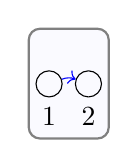
\begin{tikzpicture}
        \node at (0,0.53) {}; 
        \node at (0,0) [node, label=below:$1$] (1) {};
        \node at (.5,0) [node, label=below:$2$] (2) {};
        \draw[->, color=blue] (1) to[out=20, in=160] (2);
        %
        \pgfBox
      \end{tikzpicture}
    };
    \node[font=\scriptsize, above] at (r.north) {$R_0$};
    \path (k) edge[->] node[trans, above] {} (l);
    \path (k) edge[->] node[trans, above] {} (r);    
    \end{tikzpicture}
%  }
    %
    \hspace{1cm}
%  \hfill
  %
%  \subcaptionbox*{}{
    % RULE P1
    %
    \begin{tikzpicture}[node distance=2mm, font=\small]
      \node (l) {
      \begin{tikzpicture}
        %
        \node at (0,0.53) {}; 
        \node at (0,0) [node, label=below:$1$] (1) {} ;
        % 
      \pgfBox
      \end{tikzpicture} 
    };
    \node[font=\scriptsize, above] at (l.north) {$L_1$};
    \node [right=of l] (k) {
      
\begin{tikzpicture}
        %
        \node at (0,0.53) {}; 
        \node at (0,0) [node, label=below:$1$] (1) {};
        % 
        \pgfBox
      \end{tikzpicture} 
    };
    \node[font=\scriptsize, above] at (k.north) {$K_1$};
    \node[below] at (k.south) {$\rho_1$};
    \node  [right=of k] (r) {
      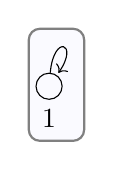
\begin{tikzpicture}
        \node at (0,0) [node, label=below:$1$] (1) {}
         edge [in=55, out=85, loop] ();
        %
        \pgfBox
      \end{tikzpicture}
    };
    \node[font=\scriptsize, above] at (r.north) {$R_1$};
    \path (k) edge[->] node[trans, above] {} (l);
    \path (k) edge[->] node[trans, above] {} (r);
    \end{tikzpicture}
%  }
  % 
    \hspace{1cm}
    %\hfill
  %
%    \subcaptionbox*{}{
    % RULE P2
    %
    \begin{tikzpicture}[node distance=2mm, font=\small]
      \node (l) {
      \begin{tikzpicture}
        %
        \node at (0,0.53) {}; 
        \node at (0,0) [node, label=below:$1$] (1) {} ;
        \node at (0.5,0) [node, label=below:$2$] (2) {} ;
      %
      \pgfBox
      \end{tikzpicture} 
    };
    \node[font=\scriptsize, above] at (l.north) {$L_2$};
    \node [right=of l] (k) {
      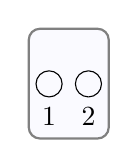
\begin{tikzpicture}
        %
        \node at (0,0.53) {}; 
        \node at (0,0) [node, label=below:$1$] (1) {} ;
        \node at (0.5,0) [node, label=below:$2$] (2) {} ;
      %
      \pgfBox
      \end{tikzpicture} 
    };
    \node[font=\scriptsize, above] at (k.north) {$K_2$};
    \node[below] at (k.south) {$\rho_2$};
    \node  [right=of k] (r) {
      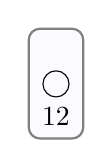
\begin{tikzpicture}
        \node at (0,0.53) {}; 
        \node at (0,0) [node, label=below:$12$] (12) {};
        %
        \pgfBox
      \end{tikzpicture}
    };
    \node[font=\scriptsize, above] at (r.north) {$R_2$};
    \path (k) edge[->] node[trans, above] {} (l);
    \path (k) edge[->] node[trans, above] {} (r);
    \end{tikzpicture}
 % }
  %
\end{center}

%%% Local Variables:
%%% mode: latex
%%% TeX-master: t
%%% End:

  
\caption{The type graph  and the rules of the grammar of the example.}
\label{fi:rules}
\end{figure}

Now, let us consider an initial graph with a single node. We can then obtain
the derivation $\rho_1 = \delta_1; \delta_2; \delta_3$ in Fig.~\ref{fi:der1}, where $\delta_2$ and $\delta_3$ are
sequential independent according to the standard notion.

\begin{figure}
    \begin{center}
    \begin{tikzpicture}[node distance=2mm, baseline=(current bounding box.center)]      
      \node (L1) at (0,2) {
        \begin{tikzpicture}
          % 
          \node at (0,0.53) {};
          \node at (0,0) [node, label=below:$1$] (1) {} ;
          % 
          \pgfBox
        \end{tikzpicture} 
      };
      \node [right=of L1] (K1) {
        
\begin{tikzpicture}
          % 
          \node at (0,0.53) {}; 
          \node at (0,0) [node, label=below:$1$] (1) {};
          % 
          \pgfBox
        \end{tikzpicture} 
      };
      \node [above=of K1] {$p_1$};
      \node [right=of K1](R1) {
        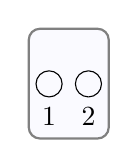
\begin{tikzpicture}
          \node at (0,0.53) {}; 
          \node at (0,0) [node, label=below:$1$] (1) {};
          \node at (.5,0) [node, label=below:$2$] (2) {}; 
          % 
          \pgfBox
        \end{tikzpicture}
      };
      \path (K1) edge[->] node[trans, above] {} (L1);
      \path (K1) edge[->] node[trans, above] {} (R1);

      \node at (4,2) (L2) {
        
\begin{tikzpicture}
          % 
          \node at (0,0.53) {}; 
          \node at (0,0) [node, label=below:$2$] (2) {} ;
          % 
          \pgfBox
        \end{tikzpicture} 
      };
      \node [right=of L2] (K2) {
        
\begin{tikzpicture}
          % 
          \node at (0,0.53) {}; 
          \node at (0,0) [node, label=below:$2$] (2) {};
          % 
          \pgfBox
        \end{tikzpicture} 
      };
      \node [above=of K2] {$p_2$};
      \node [right=of K2] (R2) {
        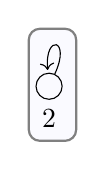
\begin{tikzpicture}
          \node at (0,0) [node, label=below:$2$] (2) {}
          edge [in=95, out=65, loop] ();        
          % 
          \pgfBox
        \end{tikzpicture}
      };
      \path (K2) edge[->] node[trans, above] {} (L2);
      \path (K2) edge[->] node[trans, above] {} (R2);

      \node at (8,2) (L3) {
        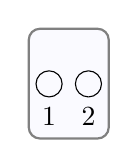
\begin{tikzpicture}
          % 
          \node at (0,0.53) {}; 
          \node at (0,0) [node, label=below:$1$] (1) {} ;
          \node at (0.5,0) [node, label=below:$2$] (2) {} ;
          % 
          \pgfBox
        \end{tikzpicture} 
      };
      \node [right=of L3] (K3) {
        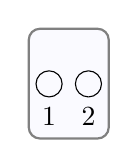
\begin{tikzpicture}
          % 
          \node at (0,0.53) {}; 
          \node at (0,0) [node, label=below:$1$] (1) {} ;
          \node at (0.5,0) [node, label=below:$2$] (2) {} ;
          % 
          \pgfBox
        \end{tikzpicture} 
      };
      \node [above=of K3] {$p_3$};
      \node [right=of K3] (R3) {
        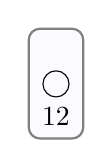
\begin{tikzpicture}
          \node at (0,0.53) {}; 
          \node at (0,0) [node, label=below:$12$] (12) {};
          % 
          \pgfBox
        \end{tikzpicture}
      };
      \path (K3) edge[->] node[trans, above] {} (L3);
      \path (K3) edge[->] node[trans, above] {} (R3);

      %%%%%% second row
      \node at (0,0) (G1) {
        
\begin{tikzpicture}
          % 
          \node at (0,0.53) {};
          \node at (0,0) [node, label=below:$1$] (1) {} ;
          % 
          \pgfBox
        \end{tikzpicture} 
      };
      \node [right=of G1] (D1) {
        
\begin{tikzpicture}
          % 
          \node at (0,0.53) {}; 
          \node at (0,0) [node, label=below:$1$] (1) {};
          % 
          \pgfBox
        \end{tikzpicture} 
      };
      \node at (3,0) (G2) {
        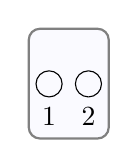
\begin{tikzpicture}
          % 
          \node at (0,0.53) {}; 
          \node at (0,0) [node, label=below:$1$] (1) {} ;
          \node at (0.5,0) [node, label=below:$2$] (2) {} ;
          % 
          \pgfBox
        \end{tikzpicture} 
      };
      \path (D1) edge[->] node[trans, above] {} (G1);
      \path (D1) edge[->] node[trans, above] {} (G2);
      \path (L1) edge[->] node[trans, above] {} (G1);
      \path (K1) edge[->] node[trans, above] {} (D1);
      \path (R1) edge[->] node[trans, above] {} (G2);

      \node at (5,0) (D2) {
        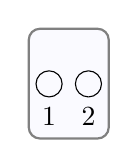
\begin{tikzpicture}
          % 
          \node at (0,0.53) {};
          \node at (0,0) [node, label=below:$1$] (1) {} ;
          \node at (0.5,0) [node, label=below:$2$] (2) {} ;                    
          % 
          \pgfBox
        \end{tikzpicture} 
      };
      \node at (7,0) (G3) {
        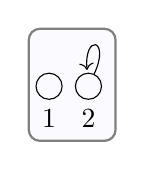
\begin{tikzpicture}
          % 
          \node at (0,0.53) {}; 
          \node at (0,0) [node, label=below:$1$] (1) {};
          \node at (0.5,0) [node, label=below:$2$] (2) {}
                edge [in=95, out=65, loop] ();                    
          % 
          \pgfBox
        \end{tikzpicture} 
      };

      \path (D2) edge[->] node[trans, above] {} (G2);
      \path (D2) edge[->] node[trans, above] {} (G3);
      \path (L2) edge[->] node[trans, above] {} (G2);
      \path (K2) edge[->] node[trans, above] {} (D2);
      \path (R2) edge[->] node[trans, above] {} (G3);
      
      \node at (9.46,0) (D3) {
        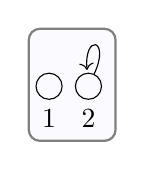
\begin{tikzpicture}
          % 
          \node at (0,0) [node, label=below:$1$] (1) {};
          \node at (0.5,0) [node, label=below:$2$] (2) {}
                edge [in=95, out=65, loop] () ;
          % 
          \pgfBox
        \end{tikzpicture} 
      };
      \node [right=of D3] (G4) {
        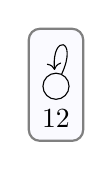
\begin{tikzpicture}
          % 
          \node at (0,0) [node, label=below:$12$] (12) {}
                edge [in=95, out=65, loop] ();
          % 
          \pgfBox
        \end{tikzpicture} 
      };

      \path (D3) edge[->] node[trans, above] {} (G3);
      \path (D3) edge[->] node[trans, above] {} (G4);
      \path (L3) edge[->] node[trans, above] {} (G3);
      \path (K3) edge[->] node[trans, above] {} (D3);
      \path (R3) edge[->] node[trans, above] {} (G4);
    \end{tikzpicture}
  %
\end{center}
%%% Local Variables:
%%% mode: latex
%%% TeX-master: t
%%% End:

\caption{The derivation $\rho_1$.}
\label{fi:der1}
\end{figure}

We can exchange the applications of $p_2$ and $p_3$, thus getting the
derivation $\rho_2 = \delta_1; \delta_3'; \delta_2'$ in
Figure~\ref{fi:der2}. Now, one can exchange again $p_3$ and $p_2$,
reaching the derivation $\rho_3 = \delta_1; \delta_2'; \delta_3$ in
Figure~\ref{fi:der3}, where in $\delta_2'$ production $p_2$ uses the
node of the start graph and thus ``does not depend'' on $p_1$.


\begin{figure}[t]
    \begin{center}
    \begin{tikzpicture}[node distance=2mm, baseline=(current bounding box.center)]      
      \node (L1) at (0,2) {
        \begin{tikzpicture}
          % 
          \node at (0,0.53) {};
          \node at (0,0) [node, label=below:$1$] (1) {} ;
          % 
          \pgfBox
        \end{tikzpicture} 
      };
      \node [right=of L1] (K1) {
        
\begin{tikzpicture}
          % 
          \node at (0,0.53) {}; 
          \node at (0,0) [node, label=below:$1$] (1) {};
          % 
          \pgfBox
        \end{tikzpicture} 
      };
      \node [above=of K1] {$p_1$};
      \node [right=of K1](R1) {
        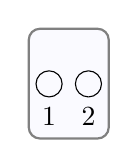
\begin{tikzpicture}
          \node at (0,0.53) {}; 
          \node at (0,0) [node, label=below:$1$] (1) {};
          \node at (.5,0) [node, label=below:$2$] (2) {}; 
          % 
          \pgfBox
        \end{tikzpicture}
      };
      \path (K1) edge[->] node[trans, above] {} (L1);
      \path (K1) edge[->] node[trans, above] {} (R1);


      \node at (4,2) (L3) {
        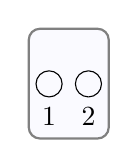
\begin{tikzpicture}
          % 
          \node at (0,0.53) {}; 
          \node at (0,0) [node, label=below:$1$] (1) {} ;
          \node at (0.5,0) [node, label=below:$2$] (2) {} ;
          % 
          \pgfBox
        \end{tikzpicture} 
      };
      \node [right=of L3] (K3) {
        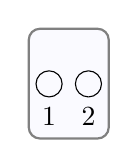
\begin{tikzpicture}
          % 
          \node at (0,0.53) {}; 
          \node at (0,0) [node, label=below:$1$] (1) {} ;
          \node at (0.5,0) [node, label=below:$2$] (2) {} ;
          % 
          \pgfBox
        \end{tikzpicture} 
      };
      \node [above=of K3] {$p_3$};
      \node [right=of K3] (R3) {
        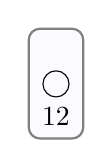
\begin{tikzpicture}
          \node at (0,0.53) {}; 
          \node at (0,0) [node, label=below:$12$] (12) {};
          % 
          \pgfBox
        \end{tikzpicture}
      };
      \path (K3) edge[->] node[trans, above] {} (L3);
      \path (K3) edge[->] node[trans, above] {} (R3);

      \node at (8,2) (L2) {
        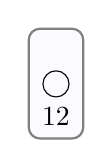
\begin{tikzpicture}
          % 
          \node at (0,0.53) {}; 
          \node at (0,0) [node, label=below:$12$] (1) {} ;
          % 
          \pgfBox
        \end{tikzpicture} 
      };
      \node [right=of L2] (K2) {
        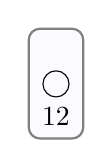
\begin{tikzpicture}
          % 
          \node at (0,0.53) {}; 
          \node at (0,0) [node, label=below:$12$] (1) {};
          % 
          \pgfBox
        \end{tikzpicture} 
      };
      \node [above=of K2] {$p_2$};
      \node [right=of K2] (R2) {
        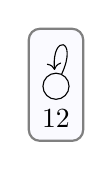
\begin{tikzpicture}
          \node at (0,0) [node, label=below:$12$] (1) {}
          edge [in=95, out=65, loop] ();        
          % 
          \pgfBox
        \end{tikzpicture}
      };
      \path (K2) edge[->] node[trans, above] {} (L2);
      \path (K2) edge[->] node[trans, above] {} (R2);

      
      %%%%%% second row
      \node at (0,0) (G1) {
        
\begin{tikzpicture}
          % 
          \node at (0,0.53) {};
          \node at (0,0) [node, label=below:$1$] (1) {} ;
          % 
          \pgfBox
        \end{tikzpicture} 
      };
      \node [right=of G1] (D1) {
        
\begin{tikzpicture}
          % 
          \node at (0,0.53) {}; 
          \node at (0,0) [node, label=below:$1$] (1) {};
          % 
          \pgfBox
        \end{tikzpicture} 
      };
      \node at (3,0) (G2) {
        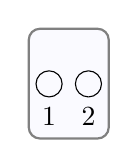
\begin{tikzpicture}
          % 
          \node at (0,0.53) {}; 
          \node at (0,0) [node, label=below:$1$] (1) {} ;
          \node at (0.5,0) [node, label=below:$2$] (2) {} ;
          % 
          \pgfBox
        \end{tikzpicture} 
      };
      \path (D1) edge[->] node[trans, above] {} (G1);
      \path (D1) edge[->] node[trans, above] {} (G2);
      \path (L1) edge[->] node[trans, above] {} (G1);
      \path (K1) edge[->] node[trans, above] {} (D1);
      \path (R1) edge[->] node[trans, above] {} (G2);

      \node at (5.5,0) (D2) {
        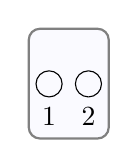
\begin{tikzpicture}
          % 
          \node at (0,0.53) {};
          \node at (0,0) [node, label=below:$1$] (1) {} ;
          \node at (0.5,0) [node, label=below:$2$] (2) {} ;                    
          % 
          \pgfBox
        \end{tikzpicture} 
      };
      \node at (7.4,0) (G3) {
        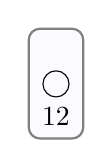
\begin{tikzpicture}
          % 
          \node at (0,0.53) {}; 
          \node at (0,0) [node, label=below:$12$] (12) {};
          % 
          \pgfBox
        \end{tikzpicture} 
      };

      \path (D2) edge[->] node[trans, above] {} (G2);
      \path (D2) edge[->] node[trans, above] {} (G3);
      \path (L3) edge[->] node[trans, above] {} (G2);
      \path (K3) edge[->] node[trans, above] {} (D2);
      \path (R3) edge[->] node[trans, above] {} (G3);
      
      \node at (9.1,0) (D3) {
        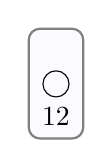
\begin{tikzpicture}
          % 
          \node at (0,0.53) {}; 
          \node at (0,0) [node, label=below:$12$] (12) {};
          % 
          \pgfBox
        \end{tikzpicture} 
      };
      \node [right=of D3] (G4) {
        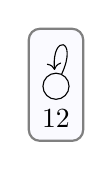
\begin{tikzpicture}
          % 
          \node at (0,0) [node, label=below:$12$] (12) {}
                edge [in=95, out=65, loop] ();
          % 
          \pgfBox
        \end{tikzpicture} 
      };

      \path (D3) edge[->] node[trans, above] {} (G3);
      \path (D3) edge[->] node[trans, above] {} (G4);
      \path (L2) edge[->] node[trans, above] {} (G3);
      \path (K2) edge[->] node[trans, above] {} (D3);
      \path (R2) edge[->] node[trans, above] {} (G4);
    \end{tikzpicture}
  %
\end{center}
%%% Local Variables:
%%% mode: latex
%%% TeX-master: t
%%% End:

\caption{The derivation $\rho_2$.}
\label{fi:der2}
\end{figure}

\begin{figure}[t]
    \begin{center}
    \begin{tikzpicture}[node distance=2mm, baseline=(current bounding box.center)]      
      \node (L1) at (0,2) {
        \begin{tikzpicture}
          % 
          \node at (0,0.53) {};
          \node at (0,0) [node, label=below:$1$] (1) {} ;
          % 
          \pgfBox
        \end{tikzpicture} 
      };
      \node [right=of L1] (K1) {
        
\begin{tikzpicture}
          % 
          \node at (0,0.53) {}; 
          \node at (0,0) [node, label=below:$1$] (1) {};
          % 
          \pgfBox
        \end{tikzpicture} 
      };
      \node [above=of K1] {$p_1$};
      \node [right=of K1](R1) {
        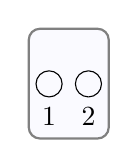
\begin{tikzpicture}
          \node at (0,0.53) {}; 
          \node at (0,0) [node, label=below:$1$] (1) {};
          \node at (.5,0) [node, label=below:$2$] (2) {}; 
          % 
          \pgfBox
        \end{tikzpicture}
      };
      \path (K1) edge[->] node[trans, above] {} (L1);
      \path (K1) edge[->] node[trans, above] {} (R1);

      \node at (4,2) (L2) {
        
\begin{tikzpicture}
          % 
          \node at (0,0.53) {}; 
          \node at (0,0) [node, label=below:$1$] (1) {} ;
          % 
          \pgfBox
        \end{tikzpicture} 
      };
      \node [right=of L2] (K2) {
        
\begin{tikzpicture}
          % 
          \node at (0,0.53) {}; 
          \node at (0,0) [node, label=below:$1$] (1) {};
          % 
          \pgfBox
        \end{tikzpicture} 
      };
      \node [above=of K2] {$p_2$};
      \node [right=of K2] (R2) {
        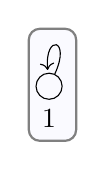
\begin{tikzpicture}
          \node at (0,0) [node, label=below:$1$] (1) {}
          edge [in=95, out=65, loop] ();        
          % 
          \pgfBox
        \end{tikzpicture}
      };
      \path (K2) edge[->] node[trans, above] {} (L2);
      \path (K2) edge[->] node[trans, above] {} (R2);

      \node at (8,2) (L3) {
        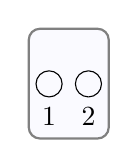
\begin{tikzpicture}
          % 
          \node at (0,0.53) {}; 
          \node at (0,0) [node, label=below:$1$] (1) {} ;
          \node at (0.5,0) [node, label=below:$2$] (2) {} ;
          % 
          \pgfBox
        \end{tikzpicture} 
      };
      \node [right=of L3] (K3) {
        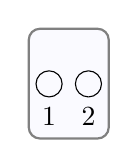
\begin{tikzpicture}
          % 
          \node at (0,0.53) {}; 
          \node at (0,0) [node, label=below:$1$] (1) {} ;
          \node at (0.5,0) [node, label=below:$2$] (2) {} ;
          % 
          \pgfBox
        \end{tikzpicture} 
      };
      \node [above=of K3] {$p_3$};
      \node [right=of K3] (R3) {
        \begin{tikzpicture}
          \node at (0,0.53) {}; 
          \node at (0,0) [node, label=below:$12$] (12) {};
          % 
          \pgfBox
        \end{tikzpicture}
      };
      \path (K3) edge[->] node[trans, above] {} (L3);
      \path (K3) edge[->] node[trans, above] {} (R3);

      %%%%%% second row
      \node at (0,0) (G1) {
        \begin{tikzpicture}
          % 
          \node at (0,0.53) {};
          \node at (0,0) [node, label=below:$1$] (1) {} ;
          % 
          \pgfBox
        \end{tikzpicture} 
      };
      \node [right=of G1] (D1) {
        \begin{tikzpicture}
          % 
          \node at (0,0.53) {}; 
          \node at (0,0) [node, label=below:$1$] (1) {};
          % 
          \pgfBox
        \end{tikzpicture} 
      };
      \node at (3,0) (G2) {
        \begin{tikzpicture}
          % 
          \node at (0,0.53) {}; 
          \node at (0,0) [node, label=below:$1$] (1) {} ;
          \node at (0.5,0) [node, label=below:$2$] (2) {} ;
          % 
          \pgfBox
        \end{tikzpicture} 
      };
      \path (D1) edge[->] node[trans, above] {} (G1);
      \path (D1) edge[->] node[trans, above] {} (G2);
      \path (L1) edge[->] node[trans, above] {} (G1);
      \path (K1) edge[->] node[trans, above] {} (D1);
      \path (R1) edge[->] node[trans, above] {} (G2);

      \node at (5,0) (D2) {
        \begin{tikzpicture}
          % 
          \node at (0,0.53) {};
          \node at (0,0) [node, label=below:$1$] (1) {} ;
          \node at (0.5,0) [node, label=below:$2$] (2) {} ;                    
          % 
          \pgfBox
        \end{tikzpicture} 
      };
      \node at (7,0) (G3) {
        \begin{tikzpicture}
          % 
          \node at (0,0.53) {}; 
          \node at (0,0) [node, label=below:$1$] (1) {}
                edge [in=95, out=65, loop] ();
          \node at (0.5,0) [node, label=below:$2$] (2) {} ;                    
          % 
          \pgfBox
        \end{tikzpicture} 
      };

      \path (D2) edge[->] node[trans, above] {} (G2);
      \path (D2) edge[->] node[trans, above] {} (G3);
      \path (L2) edge[->] node[trans, above] {} (G2);
      \path (K2) edge[->] node[trans, above] {} (D2);
      \path (R2) edge[->] node[trans, above] {} (G3);
      
      \node at (9.46,0) (D3) {
        \begin{tikzpicture}
          % 
          \node at (0,0) [node, label=below:$1$] (1) {}
                edge [in=95, out=65, loop] ();
          \node at (0.5,0) [node, label=below:$2$] (2) {} ;
          % 
          \pgfBox
        \end{tikzpicture} 
      };
      \node [right=of D3] (G4) {
        \begin{tikzpicture}
          % 
          \node at (0,0) [node, label=below:$12$] (12) {}
                edge [in=95, out=65, loop] ();
          % 
          \pgfBox
        \end{tikzpicture} 
      };

      \path (D3) edge[->] node[trans, above] {} (G3);
      \path (D3) edge[->] node[trans, above] {} (G4);
      \path (L3) edge[->] node[trans, above] {} (G3);
      \path (K3) edge[->] node[trans, above] {} (D3);
      \path (R3) edge[->] node[trans, above] {} (G4);
    \end{tikzpicture}
  %
\end{center}
%%% Local Variables:
%%% mode: latex
%%% TeX-master: t
%%% End:

\caption{The derivation $\rho_3$.}
\label{fi:der3}
\end{figure}

The fact that if we switch two steps and then switch them back, we may obtain a derivation that is not coincident with the original one has unpleasant consequences. For instance, if we restrict $\rho_1'$ and $\rho_3'$ to the first two steps, we get non-equivalent derivations $\delta_1;\delta_2 \not\shifteq \delta_1;\delta_2'$, but $\rho_1 \shifteq[\sigma] \rho_3$, with $\sigma$ mapping $\delta_1$ to $\delta_1$ and $\delta_2$ to $\delta_2'$.
%
Such a behaviour with respect to composition does not allow to obtain a causal semantics for graph transformation systems.
More precisely, it does  not allow to associate an event structure to a derivation.
%
Thus, the notion of sequential independence has to be refined. The point is that in the associated shift equivalence we want to forget who made the fusion, 
but we should not forget (as it happens in the example) that some fusions occurred.

% In Andrea's counterexample (same as above, but $p_2$ produces an item that is consumed by $p_3$, thus forcing $p_3$ to happen last), if we construct the domain we have:
% \begin{center}
%   \includegraphics[scale=.7]{dom.pdf}
% \end{center}
% which is a weak prime domain (actually a prime domain) but it does not capture the proper semantics (e.g., $p_2'$ and $p_3$ are the same event!).

Shift equivalence is made stricter by asking that two steps are
sequentially independent if the result of their switch is uniquely
determined. Intuitively, when there are several way of performing the
exchange, it means that the first step has executed some fusions that
the second step is using in an essential way, hence they should not
considered independent. Formally, this boils down to require that 
in the definition of sequential independence the interchange pair is unique.

The paper builds on this intuition: it introduces this stricter notion of sequential independence
(Section~xxx) and prove that the associated theory of shift equivalence on derivations is 
well-behaved with respect to the concatenation of rewriting steps (Section~xxx).
Finally, it outlines how the relationship with event structure works, wrapping up the paper
with comparison with related woks and hinting at further direction of research (Section~xxx).


\section{Preliminaries [to be redone]}

\begin{figure}[t]
   \begin{center}
  \begin{tikzcd}[column sep=small, row sep=normal]
    {L_1} \ar[d, "m_{L_1}" swap]
    &
    {K_1} \ar[l, "l_1" swap] \ar[r, "r_1"] \ar[d, "m_{K_1}" description]
    &
    {R_1} \ar[dr, "m_{R_1}" description]  \ar[drrr, dotted, bend left=16, "i_1" description, pos=0.75]
    & &
    % 
    {L_2}\ar[dl, "m_{L_2}" description] \ar[dlll, dotted, bend right=16, "i_2" description, pos=0.75]
    &
    {K_2} \ar[l, "l_2" swap] \ar[r, "r_2"] \ar[d, "m_{K_2}" description]
    &
    {R_2} \ar[d, "m_{R_2}"] \\
    % 
    % 
    {G}
    &
    {D_1} \ar[l, "l^*_1"] \ar[rr, "r^*_1" swap]
    & {} &
    {H}
    & {} &
    {D_2} \ar[ll, "l^*_2"] \ar[r, "r^*_2" swap]
    &
    {M}  
  \end{tikzcd}
\end{center}

%%% Local Variables:
%%% mode: latex
%%% TeX-master: ../GraphShift.tex
%%% End:

\caption{Sequential independence for
  $\rho = G \Rrel{p_1/m_1} H \Rrel{p_2/m_2} M$.}
\label{fi:strongseq}
\end{figure}


\begin{definition}[sequential independence]
  \label{de:seq-ind}
  Consider a derivation $G \Rrel{p_1/m_1} H \Rrel{p_2/m_2} M$ as in
  Fig.~\ref{fi:strongseq}. Then, its components are \emph{sequentially
    independent} if there exists a unique \emph{independence pair} among
  them, i.e., two graph morphisms $i_1: R_1 \rightarrow D_2$ and
  $i_2: L_2 \rightarrow D_1$ such that $l_2^* \circ i_1 = m_{R_1}$,
  $r_1^* \circ i_2 = m_{L_2}$.
\end{definition}

Observe that this notion reduces to the usual one for linear rules. In
fact when $r_1^*$ and $l_2^*$ are mono the uniqueness requirement is
trivially satisfied. Instead, for left-injective rules $i_1$ is still
unique, but $i_2$ might be not (as it happens, e.g., in the example
before).\todo{Say more about the example}



Observe that the notion is not symmetric: if
$\rho = G \Rrel{p_1/m_1} H \Rrel{p_2/m_2} M$ is sequential independent
and we switch it, we could obtain a pair which is not because it fails
to satisfy uniqueness of the independence pair (this happens, e.g., in
our example, where $\delta_2;\delta_3$ is sequential independent, but
$\delta_3';\delta_2'$ is not). The idea is to define shift equivalence
as $\rho \equiv_{sh} \rho'$ when \emph{each of the two} can be
obtained from the other by exchanging sequential independent
derivations. More precisely, we have a shift relation, which is used
for defining the equivalence as in Fig.~\ref{fi:ind}. It could be
better to have a slightly less elegant but more direct
definition. Write $\rho \shiftdir[\transp{i}] \rho'$ when
$\rho = \rho_1; \rho_2; \rho_3$ and $\rho' = \rho_1; \rho_2', \rho_3$
with $|\rho_1| = i-1$, $|\rho_2|=2$ and $\rho_2' \in
\IC{\rho_2}$. Then we write $\rho \shiftpre[\perm] \rho'$ if
$\rho = \rho_0 \shiftdir[\perm_1] \rho_1 \ldots \shiftdir[\perm_n ]
\rho'$ with $\perm = \perm_1; \ldots; \perm_n$ for some $n \geq 0$
(with the convention that for $n=0$ we get the identity).

The restricted notion of sequential independence ensures that the interchange operator produces a result that is unique up to abstraction equivalence.

\begin{lemma}[IC is unique]
  \label{le:unique-IC} 
  Let $\rho$ be a derivation such that $|\rho|=2$. If $\rho$ is
  sequential independent, let us write
  $\IC{\rho} = \{ \rho' \mid \rho \shiftdir \rho'\}$. Then for
  all $\rho', \rho'' \in \IC{\rho}$ we have $\rho' \equiv
  \rho''$. Moreover, if $\rho$ is sequential independent then for all
  $\rho' \in \IC{\rho}$, if $\rho'$ is sequential independent and
  $\rho'' \in \IC{\rho'}$, we have $\rho \equiv \rho''$.
\end{lemma}


\begin{figure}[t]
  \begin{center}
  \begin{tikzcd}[column sep=small, row sep=huge]
    &
    \delta_1
    &
    &[-17pt]
    &[-17pt]
    & &
    \rho
    & & &[-17pt] &[-17pt] &
    \delta_n\\[-25pt]
    %
    L_1 \arrow[d] &
    K_1 \arrow[l, tail] \arrow[r] \arrow[d] &
    R_1 \arrow[dr] \ar[drrrrrrrrr, dashed, bend left=2, "i_{1,n}" description, pos=0.6]
    &
    &
    L_2 \arrow[dl] 
    & \arrow[l, dotted, tail] \arrow[rr, dotted, no head]
    &
    & {} \arrow[r, dotted]
    &
    R_{n-1} \arrow[dr] &
    &
    L_n \arrow[dl] \ar[dlllllllll, dashed, bend right=2, "i_{n,1}" description, pos=0.6]
    &
    K_n \arrow[l, tail] \arrow[r] \arrow[d]
    &
    R_n \arrow[d]\\
    %%%%%%% 
    %%%%%%%
    G_1 &
    D_1 \arrow[l, tail] \arrow[rr] \arrow[drrrrr, dotted]
    &
    &
    G_2 \arrow[drrr, dotted]
    &
    &
    D_2 \arrow[ll, tail] \arrow[rr, no head, dotted] \arrow[dr, dotted]
    & 
    &
    D_{n-1} \arrow[dl, dotted]
    &
    &
    G_n \arrow[ll] \arrow[dlll, dotted]
    &
    &
    D_n  \arrow[ll, tail] \arrow[r] \arrow[dlllll, dotted]
    &
    G_{n+1}\\[-18pt]
    %%%%%%%
    %%%%%%%
    &
    &
    &
    &
    &    
    &
    C
    &
    &
    &
    &
    &
    &      
    % \arrow[loop below,"f_C=\cone f \bigsqcup" below]
    % \arrow[r,  "\alpha=\bigsqcup" below, shift right=1ex]
    % &
    % L \arrow[l,  "\gamma=\cone{.}" above, shift right=1ex]
    % \arrow[loop below,"f" below]
\end{tikzcd}
\end{center}

%%% Local Variables:
%%% mode: latex
%%% TeX-master: t
%%% End:

  \caption{Independence.}
  \label{fi:independence}
\end{figure}

It is convenient (at the beginning, at least) to work with shift
on derivations where the source and target graph is concrete and the
middle can be taken up to iso. I think that everything can be then
easily transferred to ctc-equivalence. We say that $\rho$ and $\rho'$
are abstract shift-equivalent and write $\rho \sim \rho'$.

A crucial observation is that independence can be defined also for non-contiguous steps.

\begin{definition}[independence]
  Let $\delta_1;\rho;\delta_n$ be a derivation as in
  Fig.~\ref{fi:independence}, where $\delta_1$ and $\delta_n$ are
  direct derivations and $\rho$ is a generic, possibly empty
  derivation. We say that $\delta_1$ and $\delta_n$ are independent if
  there is a unique independence pair $i_{n,1}$ and $i_{1,n}$
  satisfying the expected commutation, where $C$ is the colimit of the
  bottom line (excluding $G_1, G_{n+1}$).
\end{definition}

The fact that the notion of independence makes sense is proved by the following lemma, showing that the notion is preserved by the shift relation.

\begin{lemma}[independence is global]
  \label{le:seq-ind-glob1}
  The notion of independence for contiguous derivation steps
  coincides with sequential independence.

  Moreover, independence is invariant under the shift-relation, i.e.,
  \begin{itemize}
    
  \item if $\delta_1;\rho;\delta_2$ and $\rho \shiftpre \delta'$ then
    in $\delta_1;\rho;\delta_2$ the steps $\delta_1$, $\delta_2$ are
    independent iff they are in $\delta_1;\delta';\delta_2$.

  \item if $\delta_1;\rho;\delta';\delta_2$ and
    $\delta_2'; \delta'' \in \IC{\delta';\delta_2}$ then in
    $\delta_1;\rho;\delta';\delta_2$ the steps $\delta_1$ and $\delta_2$ are
    independent iff they are in $\delta_1;\rho;\delta_2'$.

  \item same as before, but with shift on the left.
  \end{itemize}
\end{lemma}

\begin{proof}
  To be done. The fact that sequential independence coincides with
  independence for contiguous derivations is easy.
\end{proof}


A \emph{permutation} on $\interval{n}$ is a bijection
$\perm : \interval{n} \to \interval{n}$. We call it a
\emph{transposition} when there are $i, j \in \interval{n}$,
$i \neq j$ such that $\sigma(i)=j$, $\sigma(j) = i$ and
$\sigma(k) = k$ otherwise. Such a transposition is normally denoted as
$\transp{i}[j]$. Whenever $j = i+1$ we call it an \emph{adjacent
  transposition}.

Given a permutation $\perm$ on $\interval{n}$, the set of inversions
of $\perm$ is
$\inv{\perm} = \{ (i,j) \mid i,j \in \interval{n-1}\ \land\ i<j\
\land\ \perm(i) > \perm(j) \}$. Clearly, $\perm$ is the identity iff
$\inv{\perm}=0$.

Now, if $\perm \neq id$ there is at least an inversion of the kind
$(i,i+1)$.  Then we have that $\perm = \transp{i}; \perm'$
with $|\inv{\perm'}| = |\inv{\perm}| -1$. Hence we can inductively
express $\perm$ as a (minimal length) composition of adjacent
transpositions.


\begin{lemma}[on permutations]
  \label{le:perm}
  Let $\perm$, $\perm'$ be permutations on $\interval{n}$ and
  $\perm = \upsilon_1; \perm'; \upsilon_2$ where $\upsilon_1$ and $\upsilon_2$
  are transpositions with $\upsilon_1 = \transp{i}[j]$ and
  $\upsilon_2 = \transp{\perm'(i)}[\perm'(j)]$. Then $\sigma =
  \sigma'$.

  Moreover, let $\upsilon_1, \upsilon_2$ be adjacent
  transpositions and $\sigma' = \upsilon_1; \ldots, \upsilon_m$ a
  minimal length decomposition of $\sigma'$ in terms of adjacent
  transpositions (that thus operate on inversions). Then, for all
  $h \in \interval{m}$ with $\upsilon_h = \transp{l}[m]$ there exists
  $k \in \interval{m}$ such that
  $\upsilon_k = \transp{\upsilon_{1,h-1}^{-1};v_1;
    \upsilon_{1,k-1}(l)}[\upsilon_{1,h-1}^{-1};v_1; \upsilon_{1,k-1}(m)]$.
\end{lemma}

\begin{proof}
  The first part is easy. The second is a consequence of the fact that
  the minimal decomposition in terms of adjacent transpositions is
  essentially unique, in the sense that it consists of exchanges of
  all the inversions. To be formalised.
\end{proof}

In words, the lemma above says that if a permutation is decomposed as $\sigma = \upsilon_1; \sigma'; \upsilon_2$ with $\sigma' = \upsilon_1'; \ldots, \upsilon_n'$, where $\upsilon_1$ and $\upsilon_2$ performs a switch and its reverse, and the inner decomposition is minimal, then we can strip the first and last switch and get a decomposition of the same permutation that performs the same switches but possibly in a different order.


\begin{lemma}[no need of useless shifts]
  \label{le:no-useless-shifts}
  Let $\rho$, $\rho'$ be direct derivations and assume
  $\rho \shiftpre[\sigma] \rho'$. Then
  $\rho = \rho_0 \shiftdir[\upsilon_1] \rho_1 \ldots \shiftdir[\upsilon_n ]
  \rho'$ where $\sigma = \upsilon_1; \ldots; \upsilon_n$ and $\upsilon_j \in \inv{\upsilon_{j,n}}$ for $j \in \{1, \ldots,n\}$.
\end{lemma}

\begin{proof}
  Let $\rho \shiftpre[\perm] \rho'$. This means that
  $\rho = \rho_0 \shiftdir[\upsilon_1] \rho_1 \ldots \shiftdir[\upsilon_n ]
  \rho'$ with $\perm = \upsilon_1; \ldots; \upsilon_n$ for some $n \geq 0$.
  
  We show that if some $\upsilon_j$ does not act on an inversion, i.e.,
  $\upsilon_j \not\in \inv{\sigma_{j,n}}$ then we can shorten the
  proof of $\rho \shiftpre[\sigma] \rho'$ of two steps. This will
  allow us to conclude that we can reduce it to a proof only acting
  on inversions, as desired.

  The key observation is that, if
  $\upsilon_j \not\in \inv{\sigma_{j,n}}$ then, intuitively, the ``same
  exchange'' must be performed in the reverse direction by some
  $\upsilon_h$ ($h>j$).  Formally, if $\upsilon_j = \transp{i}$ and
  $(i,i+1)\not\in\inv{\upsilon_{i,n}}$ then there exists $h>j$ such that
  $\upsilon_{j,h-1}(i) = \upsilon_{j,h-1}(i+1)+1$ and
  $\upsilon_h = \transp{\upsilon_{j,h-1}(i+1)}$. Among all the pairs
  $j, h$ of this kind, take one with minimal $h-i$. This means that in
  the middle all transpositions are inversions of $\upsilon_{i+1,h-1}$.

  By Lemma~\ref{le:perm}, $\upsilon_i$ and $\upsilon_h$ can be
  stripped, i.e., $\upsilon_{i,h} = \upsilon_{i+1,h-1}$. Moreover,
  again by Lemma~\ref{le:perm},
  $\upsilon_{i+1}, \ldots, \upsilon_{h-1}$ perform exchanges that were
  already done in the original proof, and thus, since independence is
  invariant under shift equivalence, as expressed by
  Lemma~\ref{le:seq-ind-glob1} they are allowed. Moreover, since by
  Lemma~\ref{le:unique-IC} the result of switching is uniquely
  determined (up to iso), the resulting derivation is the same as
  before, hence we can strip $\upsilon_{i}$ and $\upsilon_{h}$,
  and conclude.
\end{proof}  

Then we can prove that whenever $\rho \shiftpre[\perm] \rho'$, each
decomposition of $\perm$ in terms of inversions leads to a valid
derivation of $\rho'$ from $\rho$.

\begin{lemma}[independence is global/2]
  \label{le:seq-ind-glob2}
  Let $\rho$, $\rho'$ be direct derivations. Let
  $\rho \shiftpre[\perm] \rho'$, with $\perm \neq id$ and let
  $\perm = \transp{i}; \perm'$ where $(i,i+1) \in \inv{\perm}$. Then
  there exists $\rho''$ such that
  $\rho \shiftpre[\transp{i}] \rho'' \shiftpre[\perm']
  \rho'$.
\end{lemma}

\begin{proof}
  Let
  $\rho = \rho_0 \shiftdir[\upsilon_1] \rho_1 \ldots
  \shiftdir[\upsilon_n] \rho'$ where $\sigma = \upsilon_1; \ldots; \upsilon_n$ and $\upsilon_j \in \inv{\upsilon_{j,n}}$ for $j \in \{1, \ldots,n\}$, be the decomposition
  provided by Lemma~\ref{le:no-useless-shifts}.
  
  We know that steps corresponding to $i$ and $i+1$ are exchanged at
  some point, namely there is $j$ such that
  $\upsilon_j =
  \transp{\upsilon_{1,j-1}(i)}[\upsilon_{1,j-1}(i+1)]$. By
  Lemma~\ref{le:seq-ind-glob1} the steps $i$ and $i+1$ are independent
  already at the beginning and thus we can exchange them first.
  More precisely, 
  \begin{center}
    $\rho \shiftdir_{\transp{i}} \rho'' \shiftdir_{\upsilon_{1,j-1}}
    \rho_j \shiftdir_{\upsilon_{j+1,n}} \rho'$.
  \end{center}
  This can be proved by induction on $j$.
\end{proof}

\begin{lemma}[more on shift]
  \label{le:more-shift}
  if $\rho_1;\rho_1' \shiftpre[\perm | \perm'] \rho_2; \rho_2'$,
  with $|\rho_1| = |\rho_2|$ and
  $\sigma : \interval{|\rho_1|-1]} \to \interval{|\rho_2|-1]}$ then
  $\rho_1 \shiftpre[\perm] \rho_2$ and
  $\rho_1' \shiftpre[\perm'] \rho_2'$.
\end{lemma}

\begin{proof}
  The results follows by the fact that, from
  Lemma~\ref{le:no-useless-shifts}, we derive that
  \begin{center} 
    $\rho_1;\rho_1' \shiftdir[ \upsilon_1 \mid id_{[1..|\rho_1'|]}]
    \ldots \shiftdir[ \upsilon_h \mid id_{[1..|\rho_1'|]}] \rho_2;
    \rho_1' \shiftdir[ id_{[1..|\rho_1|]} \mid \upsilon_1'] \ldots
    \shiftdir[ id_{[1..|\rho_1|]} \mid \upsilon_k'] \rho_2; \rho_2'$
  \end{center}
  where $\upsilon_1; \ldots; \upsilon_h$ is a decomposition of $\perm$
  in terms of inversions and, similarly,
  $\upsilon_1'; \ldots; \upsilon_k'$ is a decomposition of
  $\perm'$. Then
  $\rho_1 \shiftdir[\upsilon_1] \ldots \shiftdir[\upsilon_h] \rho_2$
  and analogously
  $\rho_1' \shiftdir[\upsilon_1'] \ldots \shiftdir[\upsilon_k']
  \rho_2'$, which leads to the desired conclusion.
\end{proof}

\todo[inline]{Note that above we assume that $\rho_1$ and $\rho_1'$ ends in the same graph. To be formalised.}

\begin{lemma}[uniqueness of permutation]
  if $\rho \shiftpre[\perm_1] \rho'$ and
  $\rho \shiftpre[\perm_2] \rho'$ then $\perm_1 = \perm_2$. In
  particular, if $\rho_1 \shiftpre[\perm_1] \rho_1$ then $\perm_1 = id$.
\end{lemma}

\begin{proof}
  We proceed by induction on the length of the derivations
  $\ell=|\rho|=|\rho'|$ and by an inner induction on the number of
  inversions in $\sigma_1$. When $\ell = 0$, the result is
  trivial. Let us assume $\ell>0$ and let $i_1 = \sigma_1^{-1}(1)$,
  $i_2 = \sigma_2^{-1}(1)$. Let
  $L_1' \stackrel{l_1'}{\leftarrow} K_1' \stackrel{r_1'}{\rightarrow}
  R_1')$ be the rule used by the first production in $\rho'$.
  By Lemma 17(1) in the paper [the implication
  that holds] $\sigma_1$ and $\sigma_2$ are consistent permutations of
  $\rho$ into $\rho'$.
  %
  Since they are consuming, it is easy to see that
  $i_1=\sigma_1^{-1}(1)$ is uniquely determined by the (equivalence
  class) of an item in the initial graph consumed by $L_1'$ and the
  same applies to $i_2=\sigma_2^{-1}(1)$, hence we conclude that
  $i_1=i_2$.

  Now, if $i_1=i_2=1$, then $\sigma_j = \transp{1}[1] \mid \sigma_j'$
  for $j \in \{1,2\}$ and $\rho = \delta; \rho_1$,
  $\rho' = \delta; \rho_1'$ where $\delta$ is the first direct
  derivation, and $\rho_1 \shiftpre[\perm_j'] \rho_1'$ for
  $j \in \{1,2\}$. Since $|\rho_1| = \ell-1$ we conclude by inductive
  hypothesis that $\sigma_1'=\sigma_2'$ and thus $\sigma_1=\sigma_2$,
  as desired.

  If instead $i_1=i_2=i>1$, since $\transp{i_1-1}[i_1]$ is an inversion for both
   $\sigma_1$ and $\sigma_2$, by Lemma~\ref{le:seq-ind-glob2} we can
  perform such a shift first, obtaining
  \begin{center}
    $\rho \shiftdir[{\transp{i-1}[i]}] \rho_1
    \shiftpre[{\transp{i-1}[i];\sigma_1}] \rho'$
    %
    \quad and \quad
    %
    $\rho \shiftdir[{\transp{i-1}[i]}] \rho_1
    \shiftpre[{\transp{i-1}[i];\sigma_2}] \rho'$
  \end{center}
  Since ${\transp{i-1}[i];\sigma_1}$ has an inversion less than
  $\sigma_1$ we conclude by inductive hypothesis that
  ${\transp{i-1}[i];\sigma_1} ={\transp{i-1}[i];\sigma_2}$, whence
  $\sigma_1=\sigma_2$.
\end{proof}

Note that the above works also with the liberal definition of
sequential independence.

\begin{lemma}[Lemma 17(2) in the paper]
  if $\rho;\rho_1 \shiftpre[\perm] \rho; \rho_2$ then
  $\perm = id_{[1..|\rho|]} \mid \perm'$ and
  $\rho_1 \shiftpre[\perm'] \rho_2$.
\end{lemma}

\begin{proof}[skecth]
  Productions are `uniquely identified by the items they consume,
  hence productions in $\rho$ are necessarily mapped to themselves,
  i.e., $\perm = id_{[1..|\rho|]} \mid \perm'$. Then we conclude
  $\rho_1 \shiftpre[\perm'] \rho_2$ by Lemma~\ref{le:more-shift}.
\end{proof}


\begin{lemma}[Lemma 20 in the paper]
  \label{le:prop-c}
  Let $\psi$ and $\psi'$ be decorated derivations. Then the following hold:
  \begin{enumerate}
  \item
    \label{le:prop-c:1}
    Let $\psi_1, \psi_1'$ be such
    that $\psi;\psi_1 \equiv^c_{\perm} \psi';\psi_1'$ and let
    $n = | \{ j \in \interval[|\psi|]{|\psi;\psi_1|-1} \mid \perm(j)
    < |\psi'| \}|$. Then for all $\phi_2, \phi_2'$ such that
    $\psi;\phi_2 \equiv^c \psi';\phi_2'$ it holds $|\phi_2| \geq n$
    and there are $\psi_2, \psi_2',\psi_3$ such that

    \begin{itemize}
    \item $\psi;\psi_1 \equiv^c \psi;\psi_2;\psi_3$
    \item $\psi;\psi_2 \equiv^c \psi';\psi_2'$
      
    \item $|\psi_2| = n$
    
    \end{itemize}

  \item
    \label{le:prop-c:2}
    Let $\psi_1, \psi_1'$, $\psi_2, \psi_2'$ be such that
    $\psi;\psi_1 \equiv^c_{\perm_1} \psi';\psi_1'$ and
    $\psi;\psi_2 \equiv^c_{\perm_2} \psi';\psi_2'$ with $\psi_1, \psi_2$
    of minimal length. Then $\psi_1 \equiv^c_\perm \psi_2 \cdot \nu$,
    where $\nu : \target{\psi_2} \to \target{\psi_2}$ is some graph isomorphism and
    $\perm(j) = \perm_2^{-1}(\perm_1(j + |\psi|))-|\psi|$ for
    $j \in \interval[0]{|\psi_1|-1}$.    
  \end{enumerate}
\end{lemma}

\begin{proof}[sketch]  
  Point ~\ref{le:prop-c:1}: The proof should be similar to the one we have already, basing the rearrangement on Lemma~\ref{le:seq-ind-glob2}. Roughly we get $\psi;\psi_1 \equiv^c \psi_a;\psi_b;\psi_{2};\psi_{3}$ and
  $\psi';\psi_1' \equiv^c \psi_a';\psi_b';\psi_{2}';\psi_{3}'$
  with
  \begin{center}
    $\psi_a;\psi_b;\psi_{2};\psi_{3}
    \equiv^c_{\perm_a|\perm_{b2}|\perm_2}
    \psi_a';\psi_b';\psi_{2}';\psi_{3}'$
  \end{center}
  with $\perm_a$ over $\interval{|\psi_a|-1}$, $\perm_{b2}$ over
  $\interval{|\psi_b;\psi_{2}|-1}$ ``mapping $\psi_b$ to $\psi_{2}'$
  and $\psi_b'$ to $\psi_{2}$'', $\perm_3$ over
  $\interval{|\psi_2|-1}$.  We deduce by Lemma~\ref{le:more-shift}
  that $\psi_a \equiv^c_{\perm_a} \psi_a'$,
  $\psi_b;\psi_{2} \equiv^c_{\perm_{b2}} \psi_b';\psi_{2}'$ and
  $\psi_{3} \equiv^c_{\perm_3} \psi_{3}'$.
  
  Now, for all $\phi_2, \phi_2'$ such that
  $\psi;\phi_2 \equiv^c \psi';\phi_2'$ we can perform the same
  splitting and this leads to the conclusion that $|\phi| \geq n$ and
  also it can be expressed as $\psi_2;\phi_2'$, that should subsume
  also the second point.
  %
\qed
\end{proof}

% \paragraph{Note.} This does not solve the problem raised by Andrea's counterexample that still applies.

Another idea could be to try to use the inductive characterisation in Figure~\ref{fi:ind} (but I do not see how to mange the transitive rule).


\begin{figure}
  \begin{center}
    \small
  \[
    \inferL{\slab{(SH-id)}}
    {\rho \shiftpre[id] \rho}
    {}
    % 
    \hspace{0.9cm}
    % 
    \inferL{\slab{(SH-exch)}}
    {\rho \shiftpre[{\transp{1}[2]}] \rho'}
    {\rho = \upsilon_1;\upsilon_2 & \rho' \in \IC{\rho}}
  \]
  
  \[
    \inferL{\slab{(SH-comp)}}
    {\rho_1 ; \rho_2  \shiftpre[\upsilon_1 \mid \upsilon_2] \rho'_1 ;
      \rho'_2}
    {\rho_1 \shiftpre[\upsilon_1] \rho'_1, \ \rho_2 \shiftpre[\upsilon_2] 
      \rho'_2,\ \tau(\rho_1) = \perm(\rho_2)}
  \]


  \[
    % 
    % \inferL{\slab{(SH-sym)}}
    % {\rho' \shiftpre[\perm^{-1}] \rho}
    % {\rho \shiftpre[\perm] \rho'}
    % % 
    % \hspace{0.3cm}
    % 
    \inferL{\slab{(SH-tr)}}
    {\rho \shiftpre[\perm'\circ \perm] \rho''}
    {\rho \shiftpre[\perm] \rho',\ \rho' \shiftpre[\perm'], \rho''}
    %
    \hspace{0.3cm}
    \inferL{\slab{(SH-eq)}}
    {\rho' \shifteq[\perm] \rho}
    {\rho \shiftpre[\perm] \rho' & \rho' \shiftpre[\perm^{-1}] \rho}
  \]
  
  
%  \noindent
%  for $\perm_1 \mid \perm_2$ the pairing of two permutations,
%  and similarly $\sqsubseteq^c_{\perm}$ is defined inductively by
  
  \[
    \inferL{\slab{(C-abs)}}
    {\psi \equiv^c_{id} \psi'} 
    {\psi \equiv^{a} \psi'} 
    % 
    \hspace{0.3cm}
    % 
    \inferL{\slab{(C-sh)}}
    {\langle \alpha, \rho, \omega \rangle \equiv^c_{\perm} \langle \alpha, \rho', \omega \rangle} 
    {\rho \shifteq[\perm] \rho'}
    % 
    \hspace{0.3cm}
    % 
    \inferL{\slab{(C-tr)}}
    {\psi \equiv^c_{\perm' \circ \perm} \psi''}
    {
      {\psi \equiv^c_{\perm} \psi'} & 
      {\psi' \equiv^c_{\perm'} \psi''}
    }
  \]
\end{center}
\caption{Inductive definition of $\shiftpre$ and $\equiv^c$, for $\perm_1 \mid \perm_2$ the pairing of two permutations.}
\label{fi:ind}
\end{figure}


% \paragraph{Consistent $5$-tuple}. The alternative is to try to amend the notion of consistent $5$-tuple by adding some dependencies between productions and asking that they are ``preserved'' by the mapping. With the new definition I fear that it could be difficult distinguishing between dependencies arising from fusions and other, hence one should try to capture all dependencies, that will concretise in a deterministic event structure. Concretely, given $\rho = p_1 p_2 \ldots p_n$ it could be mapped to $E(\rho) = \langle \{ 1, \ldots, n\}, \vdash\rangle$ where $X \vdash i$ if there exists $\rho \equiv_\perm \rho'$ such that for all $j \in X$ it holds $j < \perm(i)$.


\section{Proving invariance of independence with respect to shift}
\newcommand{\si}{\ensuremath{\mathrel{\langle \mbox{\textsc{si}}\rangle}}}

This is the way I (AC) propose to organize the proof that sequential independence is invariant with respect to shift. I copy and update some results of the previous part. Not everything is formalized completely. 

The structure of the proof should be applicable to any notion of \emph{sequential independence} for which we can prove the following facts:

\begin{definition}[conditions on sequential independence]
\label{def:si-conditions}
\begin{enumerate}
\item \label{cond:CR} Sequential independent steps can be switched. If two consecutive steps $\delta_i$ and $\delta_{i+1}$ of a derivation $\rho$ are SI (sequential independent, written $\delta_i \si \delta_{i+1}$), then there is a constructive way to obtain a derivation $\rho'$ differing from $\rho$ only for steps $\delta'_i$ and $\delta'_{i+1}$, such that $rule(\delta_i) = rule(\delta'_{i+1})$ and $rule(\delta_{i+1}) = rule(\delta'_{i})$. In this case we write $\rho \shiftdir[i] \rho'$.

\item  \label{cond:CRdet} Switching is deterministic up to iso. If $\delta_i \si \delta_{i+1}$ in $\rho$ and $\rho \shiftdir[i] \rho'$, $\rho \shiftdir[i] \rho''$, then $\rho' \equiv \rho''$.

\item \label{cond:si-symm} Sequential independence is preserved by immediate switch. If $\delta_i \si \delta_{i+1}$ in $\rho$ and $\rho \shiftdir[i] \rho'$, then $\delta'_i \si \delta'_{i+1}$ in $\rho'$.

\item  \label{cond:si-si-iso} Switch is reversible. If $\rho \shiftdir[i] \rho'$ then $\rho' \shiftdir[i] \rho$.

\item As a consequence of the previous points, if $\rho \shiftdir[i] \rho'$ and $\rho' \shiftdir[i] \rho''$ then $\rho \equiv \rho''$.

\end{enumerate}
\end{definition}
%Given a derivation $\rho = \delta_1; \ldots ; \delta_i ; \delta_{i+1}; \ldots; \delta_n$, if $\delta_i \si \delta_{i+1}$, then
\todo[inline]{I think that all conditions are satisfied by the standard definition of SI in DPO with linear rules and by our stronger notion of SI (uniqueness of the two mediating morphism \textbf{and} same property of the switched steps) in DPO with possibly non-right-linear rules. }

\begin{proposition}[$\si$ satisfies all the conditions...]
Let's call the relation of Def.~\ref{de:seq-ind} \emph{weak sequential independence}. Then it satisfies conditions \ref{cond:CR} and \ref{cond:CRdet} of Definition~\ref{def:si-conditions} (by the classical Church-Rosser Theorem and uniqueness of the mediating morphisms), but not the remaining ones. 

Let \emph{sequential independence} be defined as follows: $\delta_i \si \delta_{i+1}$ in $\rho$ iff they are weak sequential independent, and if $\rho'$ is obtained by $\rho$ switching  $\delta_i$ and $\delta_{i+1}$ (which is possible by condition \ref{cond:CR} and deterministic up to iso by condition \ref{cond:CRdet}) then $\delta'_i$ and $\delta'_{i+1}$ are weak sequential independent in $\rho'$.
 
 Then $\si$ satisfies all the conditions of Definition~\ref{def:si-conditions}.
 \end{proposition}
 
\begin{proof}
Conditions  \ref{cond:CR} and \ref{cond:CRdet} already hold for weak sequential independence. Condition \ref{cond:si-symm} holds by definition. \textbf{Condition \ref{cond:si-si-iso} should be proved explicitly, I fear...}
\end{proof}


\begin{definition}[Invariance under shift]
\label{def:invariance} 
A binary relation $R$ on consecutive steps of derivations is \emph{invariant under shift equivalence up to $n$} if whenever  $\rho = \rho_0 \shiftdir[\upsilon_1] \rho_1 \ldots \shiftdir[\upsilon_k] \rho'$ with  $\perm = \upsilon_1; \ldots; \upsilon_k$ and $k \leq n$ (thus $\rho \shifteq[\perm] \rho'$ with a proof made of at most  $n$ switches of steps) and $\perm(i+1) = \perm(i) + 1$, then $\delta_i \mathrel{R} \delta_{i+1}$ in $\rho$ if and only if $\delta'_{\perm(i)} \mathrel{R} \delta'_{\perm(i+1)}$ in $\rho'$. Relation $R$  is \emph{invariant under shift equivalence}, tout-court, if it is so up to any $n$.

In words, two consecutive steps are related by $R$ in a derivation iff they are related by $R$ in any shift-equivalent derivation in which they are again consecutive. 


%$\delta_i \mathrel{R} \delta_{i+1}$ in $\rho$, $\rho \shifteq[\perm] \rho'$, and $\perm(i+1) = \perm(i) + 1$, then $\delta'_{\perm(i)} \mathrel{R} \delta'_{\perm(i+1)}$ in $\rho'$.

\end{definition}

\todo[inline]{The following is Lemma~\ref{le:no-useless-shifts} with a bound $n$ on the length of the proof that two derivations are shift equivalent. Also, it uses as assumption the fact that \si is invariant w.r.t.~shift up to $n-1$: the fact that $n-1$ is sufficient is exploited later in the proof of the main result. I think that it works, because the assumption is used only at the end, when the two reverse transpositions were already stripped, thus the length is $n-2$.}
\begin{lemma}[no need of useless shifts]
  \label{le:no-useless-shifts-bounded}
  Given an integer $n$, let us assume that $\si$ is invariant under shift up to $n-1$.  Let $\rho$, $\rho'$ be direct derivations such that  $\rho = \rho_0 \shiftdir[\upsilon_1] \rho_1 \ldots \shiftdir[\upsilon_k] \rho'$ with $k \leq n$, and 
  let $\sigma = \upsilon_1; \ldots; \upsilon_k$.
   Then
  $\rho = \rho_0 \shiftdir[\upsilon'_1] \rho_1 \ldots \shiftdir[\upsilon'_h ]
  \rho'$ where $\sigma = \upsilon'_1; \ldots; \upsilon'_h$, $h \leq k$ and $\upsilon'_j \in \inv{\upsilon'_{j,h}}$ for $j \in \{1, \ldots,h\}$. 
  %\todo{I understand that $\upsilon'_{j,h} = \upsilon'_j; \ldots; \upsilon'_h$}
\end{lemma}

\begin{proof}
  Let 
  $\rho = \rho_0 \shiftdir[\upsilon_1] \rho_1 \ldots \shiftdir[\upsilon_k ]
  \rho'$.
  %
  We show that if some $\upsilon_j$ does not act on an inversion, i.e.,
  $\upsilon_j \not\in \inv{\upsilon_{j,k}}$ then we can shorten the
  proof of $\rho \shifteq[\sigma] \rho'$ of two steps. This 
  allow us to conclude that we can reduce the original proof to one which is not longer and only acting
  on inversions, as desired.

  The key observation is that, if
  $\upsilon_j \not\in \inv{\sigma_{j,k}}$ then, intuitively, the ``same
  exchange'' must be performed in the reverse direction by some
  $\upsilon_s$, with $s>j$.  Formally, if $\upsilon_j = \transp{i}$ and
  $(i,i+1)\not\in\inv{\upsilon_{i,k}}$ then there exists $s>j$ such that
  $\upsilon_{j,s-1}(i) = \upsilon_{j,s-1}(i+1)+1$ and
  $\upsilon_s = \transp{\upsilon_{j,s-1}(i+1)}$. Among all the pairs
  $j, s$ of this kind, take one with minimal $s-j$. This means that in
  the middle all transpositions are inversions of $\upsilon_{j+1,s-1}$.

  By Lemma~\ref{le:perm}, $\upsilon_j$ and $\upsilon_s$ can be
  stripped, i.e., $\upsilon_{j,s} = \upsilon_{j+1,s-1}$. Moreover,
  again by Lemma~\ref{le:perm},
  $\upsilon_{i+1}, \ldots, \upsilon_{s-1}$ perform exchanges that were
  already done in the original proof, and thus, since independence is
  invariant under shift equivalence up to $n-1$, they are allowed. 
  Moreover, since by condition \ref{cond:CRdet} of Definition~\ref{def:si-conditions} the result of switching is uniquely
  determined (up to iso), the resulting derivation is the same as
  before, hence we can strip $\upsilon_{j}$ and $\upsilon_{s}$,
  and conclude.
\end{proof}  

\todo[inline]{The next one is Lemma~\ref{le:seq-ind-glob2}, again bounded w.r.t.~ the length of the proof of shift equivalence. \textbf{Note:} It is not used in the following.}

Then we can prove that whenever $\rho \shifteq[\perm] \rho'$, each
decomposition of $\perm$ in terms of inversions leads to a valid
valid proof of the shift equivalence  of $\rho$ and $\rho$.

\begin{lemma}[independence is global/2]
  \label{le:seq-ind-glob2-new}
 Given an integer $n$, let us assume that $\si$ is invariant under shift up to $n$.  Let $\rho$, $\rho'$ be direct derivations such that $\rho = \rho_0 \shiftdir[\upsilon_1] \rho_1 \ldots
  \shiftdir[\upsilon_k] \rho'$, with $0 < k \leq n$,  
   $\sigma = \upsilon_1; \ldots; \upsilon_k$  and  $\upsilon_j \in \inv{\upsilon_{j,k}}$ for $j \in \{1, \ldots,k\}$. 
  Let
  $\perm = \transp{i}; \perm'$ where $(i,i+1) \in \inv{\perm}$. Then
  there exists $\rho''$ such that
  $\rho \shifteq[\transp{i}] \rho'' \shifteq[\perm']
  \rho'$.
\end{lemma}

\begin{proof}
%  Let
%  $\rho = \rho_0 \shiftdir[\upsilon_1] \rho_1 \ldots
%  \shiftdir[\upsilon_n] \rho'$ where $\sigma = \upsilon_1; \ldots; \upsilon_n$ and $\upsilon_j \in \inv{\upsilon_{j,n}}$ for $j \in \{1, \ldots,n\}$, be the decomposition
%  provided by Lemma~\ref{le:no-useless-shifts}.
 % 
  We know that steps corresponding to $i$ and $i+1$ are exchanged at
  some point, namely there is $j$ such that
  $\upsilon_j =
  \transp{\upsilon_{1,j-1}(i)}[\upsilon_{1,j-1}(i+1)]$. Since $\si$ is invariant up to $n$, the steps $i$ and $i+1$ are independent
  already at the beginning and thus we can exchange them first.
  More precisely, 
  \begin{center}
    $\rho \shiftdir_{\transp{i}} \rho'' \shiftdir_{\upsilon_{1,j-1}}
    \rho_j \shiftdir_{\upsilon_{j+1,k}} \rho'$.
  \end{center}
  This can be proved by induction on $j$.
\end{proof}

The following main lemma needs a proof. 

\begin{lemma}[Invariance of $\si$ under immediate shift]
\label{le:invariance-immediate}
\begin{enumerate}
%\item Let $\rho = \delta_1 ; \delta_2 ; \delta_3 $ with $\delta_2 \si \delta_3$, suppose that $\rho \shiftdir[(2,3)] \rho' = \delta_1 ; \delta'_3 ; \delta'_2$,  that $\delta_1 \si \delta'_3$ in $\rho'$, and that $\rho' \shiftdir[(1,2)] \rho'' =  \delta''_3 ; \delta'_1 ; \delta'_2$. 
%Then $\delta_1 \si \delta_2$ in $\rho$ if and only if  $\delta'_1 \si \delta'_2$ in $\rho''$. 

\item Let $\rho = \delta_1 ; \delta_2 ; \delta_3 $ be a derivation such that $\rho \shiftdir[(2,3)] \rho'  \shiftdir[(1,2)] \rho''$,  with $\delta_2 \si \delta_3$ in $\rho$, $\rho' = \delta_1 ; \delta'_3 ; \delta'_2$,   $\delta_1 \si \delta'_3$ in $\rho'$, and that $\rho'' =  \delta''_3 ; \delta'_1 ; \delta'_2$. 
Then $\delta_1 \si \delta_2$ in $\rho$ if and only if  $\delta'_1 \si \delta'_2$ in $\rho''$. 

The situation can be represented as in the following diagram, where each transposition is performed, downwards, only if the two starting steps are sequential independent. The proposition states that the steps \cycl{1} are sequential independent if and only if so are the steps \cycl{2}. For brevity, we abbreviate this statement to $SI(\cycl{1}) \iff SI(\cycl{2})$.

%\center{\xymatrix@C=2pc@R=1pc{
% \rho  \ar@{~>}[d]^{sh}_{(2,3)}  \ar@{}[r]|{=} & \rho_1 \ar@{-}[d] \ar@{}[r]|{;} & \delta_1 \ar@{-}[d]  \ar@{}[r]|{;} & \delta_2 \ar@{-}[dr]  \ar@{}[r]|{;} & \delta_3 \ar@{-}[dl]  \ar@{}[r]|{;} &\rho_2 \ar@{-}[d] \\
%\rho'  \ar@{~>}[d]^{sh}_{(1,2)}  \ar@{}[r]|{=} &  \rho_1 \ar@{-}[d]  \ar@{}[r]|{;} & \delta_1 \ar@{-}[dr]  \ar@{}[r]|{;} & \delta'_3 \ar@{-}[dl]  \ar@{}[r]|{;} & \delta'_2 \ar@{-}[d]  \ar@{}[r]|{;} &\rho_2 \ar@{-}[d] \\
%\rho''  \ar@{}[r]|{=} &   \rho_1 \ar@{}[r]|{;} & \delta''_3 \ar@{}[r]|{;} & \delta'_1 \ar@{}[r]|{;} & \delta'_2 \ar@{}[r]|{;} &\rho_2\\
%}}

$$\xymatrix@C=2pc@R=1pc{
 \rho  \ar@{~>}[d]^{sh}_{(2,3)}  \ar@{}[r]|{=} &  \delta_1 \ar@{-}[d]  \ar@{}[r]|{;}  \ar@{-}@/^3ex/[r]|{\cycl{1}} & \delta_2 \ar@{-}[dr]  \ar@{}[r]|{;} & \delta_3 \ar@{-}[dl] \\
\rho'  \ar@{~>}[d]^{sh}_{(1,2)}  \ar@{}[r]|{=} &   \delta_1 \ar@{-}[dr]  \ar@{}[r]|{;} & \delta'_3 \ar@{-}[dl]  \ar@{}[r]|{;} & \delta'_2 \ar@{-}[d]\\
\rho''  \ar@{}[r]|{=} &    \delta''_3 \ar@{}[r]|{;} & \delta'_1 \ar@{-}@/_3ex/[r]|{\cycl{2}} \ar@{}[r]|{;} & \delta'_2  \\
}$$




\item  Also a symmetric statement holds, for which we show only the graphical representation. Again, we show that $SI(\cycl{1}) \iff SI(\cycl{2})$.
% the steps \cycl{1} are sequential independent if and only if so are the steps \cycl{2}.



$$\xymatrix@C=2pc@R=1pc{
 \rho  \ar@{~>}[d]^{sh}_{(1,2)}  \ar@{}[r]|{=} &
   \delta_1 \ar@{-}[dr]  \ar@{}[r]|{;}  &
    \delta_2 \ar@{-}[dl]  \ar@{}[r]|{;} \ar@{-}@/^3ex/[r]|{\cycl{1}} &
    \delta_3 \ar@{-}[d] \\
\rho'  \ar@{~>}[d]^{sh}_{(2,3)}  \ar@{}[r]|{=} &
   \delta'_2 \ar@{-}[d]  \ar@{}[r]|{;} &
    \delta'_1 \ar@{-}[dr]  \ar@{}[r]|{;} &
     \delta_3 \ar@{-}[dl]\\
\rho''  \ar@{}[r]|{=} & 
   \delta'_2 \ar@{}[r]|{;} \ar@{-}@/_3ex/[r]|{\cycl{2}} &
    \delta'_3  \ar@{}[r]|{;} &
     \delta''_1  \\
}$$


%
%Symmetrically, let $\rho = \rho_1 ; \delta_1 ; \delta_2 ; \delta_3 ; \rho_2$ with $\delta_1 \si \delta_2$ in $\rho$, suppose that $\rho \shiftdir[(1,2)] \rho' = \rho_1 ; \delta'_2 ; \delta'_1 ; \delta_3 ;\rho_2$,  that $\delta'_1 \si \delta_3$ in $\rho'$, and that $\rho' \shiftdir[(2,3)] \rho'' = \rho_1 ; \delta'_2 ; \delta'_3 ; \delta''_1 ;\rho_2$. 
%Then $\delta_2 \si \delta_3$ in $\rho$ if and only if  $\delta'_2 \si \delta'_3$ in $\rho''$. 
\end{enumerate}
%\begin{enumerate}
%\item Let $\rho = \rho_1 ; \delta_1 ; \delta_2 ; \delta_3 ; \rho_2$ with $\delta_2 \si \delta_3$ in $\rho$, suppose that $\rho \shiftdir[(2,3)] \rho' = \rho_1 ; \delta_1 ; \delta'_3 ; \delta'_2 ;\rho_2$,  that $\delta_1 \si \delta'_3$ in $\rho'$, and that $\rho' \shiftdir[(1,2)] \rho'' = \rho_1 ; \delta''_3 ; \delta'_1 ; \delta'_2 ;\rho_2$. 
%Then $\delta_1 \si \delta_2$ in $\rho$ if and only if  $\delta'_1 \si \delta'_2$ in $\rho''$. 
%
%The following A graphical representation The situation can 
%\item  Symmetrically, let $\rho = \rho_1 ; \delta_1 ; \delta_2 ; \delta_3 ; \rho_2$ with $\delta_1 \si \delta_2$ in $\rho$, suppose that $\rho \shiftdir[(1,2)] \rho' = \rho_1 ; \delta'_2 ; \delta'_1 ; \delta_3 ;\rho_2$,  that $\delta'_1 \si \delta_3$ in $\rho'$, and that $\rho' \shiftdir[(2,3)] \rho'' = \rho_1 ; \delta'_2 ; \delta'_3 ; \delta''_1 ;\rho_2$. 
%Then $\delta_2 \si \delta_3$ in $\rho$ if and only if  $\delta'_2 \si \delta'_3$ in $\rho''$. 
%\end{enumerate}
\end{lemma}
\begin{proof}
\textbf{To be done...}

\end{proof}

We are now able to state and prove the main result.

\begin{theorem}[Invariance of $\si$]
Relation $\si$ is invariant under shift equivalence, as for Definition~\ref{def:invariance}.
\end{theorem}

\begin{proof}
Let $\rho \shifteq[\perm] \rho'$ be two shift equivalent derivations and let $1 \leq i <  |\rho|$ such that $\perm(i+1) = \perm(i) + 1$. We have to show that $\delta_i \si \delta_{i+1}$ in $\rho$  iff  $\delta_{\perm(i)} \si \delta_{\perm(i+1)}$ in $\rho'$.

Since $\rho \shifteq[\perm] \rho'$, we have $\rho = \rho_0 \shiftdir[\upsilon_1] \rho_1 \ldots \shiftdir[\upsilon_n] \rho'$, with $\sigma = \upsilon_1; \ldots; \upsilon_n$. We proceed by induction on $n$. If $n = 0$, then $\perm = id$ and the statement trivially holds. Now we assume that the statement holds for each $k \leq n$, and  we show that it holds for $n+1$. Let  $\sigma'$ be defined as $\sigma' =  \upsilon_1; \ldots; \upsilon_n$, thus  $\sigma = \sigma' ; \upsilon_{n+1}$.  We proceed by case analysis on the last adjacent transposition $\upsilon_{n+1} = (z, z+1)$.

\begin{description} 
\item [{[$z+1 < \sigma'(i)$ or $\sigma'(i+1) < z$]}] In this case the last transposition does not affect the steps $\delta^n_{\sigma'(i)}$ and $\delta^n_{\sigma'(i+1)}$  of $\rho_n$, as depicted here:

$$\xymatrix@C=2pc@R=2pc{
 \rho  \ar@{~>}[d]^{sh}^(.9){*} \ar@{}[r]|{=} &
   \cdots   \ar@{}[r]|{;}  &
    \delta_i \ar@{--}@/_2ex/[d]  \ar@{}[r]|{;} \ar@{-}@/^3ex/[r]|{\cycl{1}} &
    \delta_{i+1} \ar@{--}@/^1ex/[d]  \ar@{}[r]|{;}  & \cdots\\
\rho_n  \ar@{~>}[d]^{sh}_{\upsilon_{n+1}}  \ar@{}[r]|{=} &
   \cdots   \ar@{}[r]|{;}  &
    \delta^n_{\sigma'(i)} \ar@{-}[d]  \ar@{}[r]|{;}  \ar@{-}@/_3ex/[r]|{\cycl{3}}  &
   \delta^n_{\sigma'(i+1)} \ar@{-}[d]  \ar@{}[r]|{;} &
    \cdots\\
\rho'  \ar@{}[r]|{=} & 
    \cdots   \ar@{}[r]|{;}  &
     \delta'_{\sigma(i)} \ar@{}[r]|{;} \ar@{-}@/_3ex/[r]|{\cycl{2}} &
    \delta'_{\sigma(i+1)}  \ar@{}[r]|{;} &
     \cdots  \\
}$$

\todo[inline]{But is it obvious that if two steps keep their position the remain shift-equivalent? Maybe this is another condition...}
 
Therefore clearly $SI(\cycl{2}) \iff SI(\cycl{3})$. Furthermore $SI(\cycl{1}) \iff SI(\cycl{3})$  by induction hypothesis, because $\rho  \stackrel{sh\ *}{\rightsquigarrow} \rho_n$  has length $n$, and thus we conclude $SI(\cycl{1}) \iff SI(\cycl{2})$.

\item  [{[$z = \sigma'(i+1)$ and $\sigma'(i) = z+1$]}]  In this case the last transposition switches the steps $\delta^n_{\sigma'(i+1)}$ and $\delta^n_{\sigma'(i)}$  of $\rho_n$, as depicted here:


$$\xymatrix@C=2pc@R=2pc{
 \rho  \ar@{~>}[d]^{sh}^(.9){*} \ar@{}[r]|{=} &
   \cdots   \ar@{}[r]|{;}  &
    \delta_i \ar@{--}[dr]  \ar@{}[r]|{;} \ar@{-}@/^3ex/[r]|{\cycl{1}} &
    \delta_{i+1} \ar@{--}[dl]  \ar@{}[r]|{;}  & \cdots\\
\rho_n  \ar@{~>}[d]^{sh}_{\upsilon_{n+1}}  \ar@{}[r]|{=} &
   \cdots   \ar@{}[r]|{;}  &
    \delta^n_{\sigma'(i+1)} \ar@{-}[dr]  \ar@{}[r]|{;}  \ar@{-}@/^2ex/[r]|{\cycl{3}}  &
   \delta^n_{\sigma'(i)} \ar@{-}[dl]  \ar@{}[r]|{;} &
    \cdots\\
\rho'  \ar@{}[r]|{=} & 
    \cdots   \ar@{}[r]|{;}  &
     \delta'_{\sigma(i)} \ar@{}[r]|{;} \ar@{-}@/_3ex/[r]|{\cycl{2}} &
    \delta'_{\sigma(i+1)}  \ar@{}[r]|{;} &
     \cdots  \\
}$$

Clearly we have $SI(\cycl{3})$ because the two steps are switched, and thus also $SI(\cycl{2})$ by  conditions  \ref{cond:si-symm} and \ref{cond:si-si-iso} of Definition~\ref{def:si-conditions}. Furthermore, as evident from the drawing the steps $\delta_i$ and $\delta_{i+1}$ of $\rho$ must have been switched by a transposition $\upsilon_j = (v, v+1)$ with $1 \leq j \leq n$.  Therefore we have that steps $\delta^{j-1}_v$ and $\delta^{j-1}_{v+1}$  are sequential independent in $\rho^{j-1}$, and by induction hypothesis  (because $j \leq n$) we infer $SI(\cycl{1})$, allowing us to conclude that $SI(\cycl{1}) \iff SI(\cycl{2})$.
 
\item  [{[$z+1 = \sigma'(i+1)$, thus $z = \sigma(i+1)$]}]  

% and $z =\sigma'(v) for $v \gt i+1
In this case the transposition $\upsilon_{n+1}$ affects one of the steps \cycl{2} but not both, as summarized in the drawing.
$$\xymatrix@C=2pc@R=2pc{
 \rho  \ar@{~>}[d]^{sh}^(.9){*} \ar@{}[r]|{=} &
   \cdots   \ar@{}[r]|{;}  &
    \delta_i \ar@{--}@/_2ex/[d]  \ar@{}[r]|{;} \ar@{-}@/^3ex/[r]|{\cycl{1}} &
    \delta_{i+1} \ar@{--}@/^1ex/[dr]  \ar@{}[r]|{;}  & \cdots\\
\rho_n  \ar@{~>}[d]^{sh}_{\upsilon_{n+1}}  \ar@{}[r]|{=} &
   \cdots   \ar@{}[r]|{;}  &
    \delta^n_{\sigma'(i)} \ar@{-}[d]  \ar@{}[r]|{;}   &
   \delta^n_z \ar@{-}[dr]  \ar@{}[r]|{;} &
   \delta^n_{\sigma'(i+1)} \ar@{-}[dl]  \ar@{}[r]|{;} &
    \cdots\\
\rho'  \ar@{}[r]|{=} & 
    \cdots   \ar@{}[r]|{;}  &
     \delta'_{\sigma(i)} \ar@{}[r]|{;} \ar@{-}@/_3ex/[r]|{\cycl{2}} &
    \delta'_{\sigma(i+1)}  \ar@{}[r]|{;} &
    \delta'_{z+1}  \ar@{}[r]|{;} &
     \cdots  \\
}$$

There are two subcases, depending on whether step $\delta_z^n$ originates from a step in $\rho$ after $\delta_{i+1}$ or before $\delta_i$. In the first case we have:  
$$\xymatrix@C=2pc@R=2pc{
 \rho  \ar@{~>}[d]^{sh}^(.9){*} \ar@{}[r]|{=} &
   \cdots   \ar@{}[r]|{;}  &
    \delta_i \ar@{--}@/_2ex/[d]  \ar@{}[r]|{;} \ar@{-}@/^3ex/[r]|{\cycl{1}} &
   \delta_{i+1}  \ar@{--}@/^1ex/[dr]  \ar@{}[r]|{\cdots}  &
    \delta_{{\sigma'}^{-1}(z)} \ar@{--}@/_1ex/[dl]  \ar@{}[r]|{;}  & \cdots\\
\rho_n  \ar@{~>}[d]^{sh}_{\upsilon_{n+1}}  \ar@{}[r]|{=} &
   \cdots   \ar@{}[r]|{;}  &
    \delta^n_{\sigma'(i)} \ar@{-}[d]  \ar@{}[r]|{;}   &
   \delta^n_z \ar@{-}[dr]  \ar@{}[r]|{;} &
   \delta^n_{\sigma'(i+1)} \ar@{-}[dl]  \ar@{}[r]|{;} &
    \cdots\\
\rho'  \ar@{}[r]|{=} & 
    \cdots   \ar@{}[r]|{;}  &
     \delta'_{\sigma(i)} \ar@{}[r]|{;} \ar@{-}@/_3ex/[r]|{\cycl{2}} &
    \delta'_{\sigma(i+1)}  \ar@{}[r]|{;} &
    \delta'_{z+1}  \ar@{}[r]|{;} &
     \cdots  \\
}$$

As evident form the drawing, in this case there are certainly some useless transpositions. Thus by Lemma~\ref{le:no-useless-shifts-bounded} (used on proofs of length at most $n+1$, with the induction hypothesis up to length $n$) there exists an equivalent proof of $\rho \shifteq[\perm] \rho'$  of length at most $n-1$, thus we can conclude by inductive hypothesis. 

The second case is depicted as follows:

$$\xymatrix@C=2pc@R=2pc{
 \rho  \ar@{~>}[d]^{sh}^(.9){*} \ar@{}[r]|{=} &
   \delta_{{\sigma'}^{-1}}(z)  \ar@{--}@/^1ex/[drr]   \ar@{}[r]|{\cdots}  &
    \delta_i \ar@{--}@/_2ex/[d]  \ar@{}[r]|{;} \ar@{-}@/^3ex/[r]|{\cycl{1}} &
    \delta_{i+1} \ar@{--}@/^1ex/[dr]  \ar@{}[r]|{;}  & \cdots\\
\rho_n  \ar@{~>}[d]^{sh}_{\upsilon_{n+1}}  \ar@{}[r]|{=} &
   \cdots   \ar@{}[r]|{;}  &
    \delta^n_{\sigma'(i)} \ar@{-}[d]  \ar@{}[r]|{;}   &
   \delta^n_z \ar@{-}[dr]  \ar@{}[r]|{;} &
   \delta^n_{\sigma'(i+1)} \ar@{-}[dl]  \ar@{}[r]|{;} &
    \cdots\\
\rho'  \ar@{}[r]|{=} & 
    \cdots   \ar@{}[r]|{;}  &
     \delta'_{\sigma(i)} \ar@{}[r]|{;} \ar@{-}@/_3ex/[r]|{\cycl{2}} &
    \delta'_{\sigma(i+1)}  \ar@{}[r]|{;} &
    \delta'_{z+1}  \ar@{}[r]|{;} &
     \cdots  \\
}$$

We see that two steps from which $\delta^n_{\sigma'(i)}$ and $\delta^n_z$ originate were switched by a transposition $\upsilon_j$ with $1 \leq j \leq n$ therefore by induction hypothesis we infer that  $\delta^n_{\sigma'(i)}$ and $\delta^n_z$ are sequentially independent. Thus we can modify the proof as follows, switching such steps twice:
 
$$\xymatrix@C=2pc@R=2pc{
 \rho  \ar@{~>}[d]^{sh}^(.9){*} \ar@{}[r]|{=} &
   \delta_{{\sigma'}^{-1}}(z)  \ar@{--}@/^1ex/[drr]   \ar@{}[r]|{\cdots}  &
    \delta_i \ar@{--}@/_2ex/[d]  \ar@{}[r]|{;} \ar@{-}@/^3ex/[r]|{\cycl{1}} &
    \delta_{i+1} \ar@{--}@/^1ex/[dr]  \ar@{}[r]|{;}  & \cdots\\
\rho_n  \ar@{~>}[d]^{sh}_{\upsilon_{n+1}}  \ar@{}[r]|{=} &
   \cdots   \ar@{}[r]|{;}  &
    \delta^n_{\sigma'(i)} \ar@{-}[dr]  \ar@{}[r]|{;}   &
   \delta^n_z \ar@{-}[dl]  \ar@{}[r]|{;} &
   \delta^n_{\sigma'(i+1)} \ar@{-}[d]  \ar@{}[r]|{;} &
    \cdots\\
  \rho_{n+1}  \ar@{~>}[d]^{sh}_{\upsilon_{n+2}}  \ar@{}[r]|{=} &
   \cdots   \ar@{}[r]|{;}  &
    \delta^{n+1}_{z-1} \ar@{-}[dr]  \ar@{}[r]|{;}   &
   \delta^{n+1}_{\sigma'(i)+1}  \ar@{-}[dl]  \ar@{}[r]|{;}   \ar@{-}@/^3ex/[r]|{\cycl{3}} &
   \delta^{n+1}_{\sigma'(i+1)} \ar@{-}[d]  \ar@{}[r]|{;} &
    \cdots\\
    \rho_{n+2}  \ar@{~>}[d]^{sh}_{\upsilon_{n+3}}  \ar@{}[r]|{=} &
   \cdots   \ar@{}[r]|{;}  &
    \delta^{n+2}_{\sigma'(i)} \ar@{-}[d]  \ar@{}[r]|{;}   &
   \delta^{n+2}_z \ar@{-}[dr]  \ar@{}[r]|{;} &
   \delta^{n+2}_{\sigma'(i+1)} \ar@{-}[dl]  \ar@{}[r]|{;} &
    \cdots\\  
\rho'  \ar@{}[r]|{=} & 
    \cdots   \ar@{}[r]|{;}  &
     \delta'_{\sigma(i)} \ar@{}[r]|{;} \ar@{-}@/_3ex/[r]|{\cycl{2}} &
    \delta'_{\sigma(i+1)}  \ar@{}[r]|{;} &
    \delta'_{z+1}  \ar@{}[r]|{;} &
     \cdots  \\
}$$

Now we can conclude observing that $SI(\cycl{2}) \iff SI(\cycl{3})$ by point 2 of Lemma~\ref{le:invariance-immediate}, and that $SI(\cycl{1}) \iff SI(\cycl{3})$ can be proved by applying the first subcase of this step of the proof.

\todo[inline]{Lemma~\ref{le:invariance-immediate} considera solo derivazioni di lunghezza 3. Anche qui serve un lemma che garantisce che vale anche in un contesto piu' ampio.}

\item   [{[$z = \sigma'(i)$, thus $z+1 = \sigma(i)$]}]  
This case is completely symmetrical to the previous one, exploiting in the last subcase point 1 of Lemma~\ref{le:invariance-immediate}. 

\end{description}

\end{proof}

\bibliographystyle{splncs04}
%\bibliographystyle{plainurl}
\bibliography{Unstable}

\end{document}


%%% Local Variables:
%%% mode: latex
%%% TeX-master: t
%%% End:
